\documentclass[compress]{beamer}
\usepackage{etex}

%\usepackage{subfigure}
\mode<presentation>
{
 \usetheme{IARC}
}
%\setbeamersize{head/foot 5.5cm}

\usepackage{colortbl}
%\usepackage[table]{xcolor}
%\usepackage[utf8]{inputenc}
\usepackage[english]{babel}
%\usepackage{amsfonts,amsmath}
\usepackage{amssymb}
%\usepackage{empheq}%\usepackage{empheq}
%\usepackage[dvips]{graphics}
\usepackage{epsfig}
\usepackage{geometry}
%\usepackage{subfigure}
\usepackage{wrapfig}
\usepackage{subfig}
\usepackage[bottom]{footmisc}

\usepackage{appendixnumberbeamer}

%\usepackage{paralist}

%\usepackage{unnumberedcaption}
\usepackage{graphics}
\usepackage{graphicx}
%\usepackage{rotating}
\usepackage{amsmath,supertabular,tabularx}
\usepackage{multirow}
\usepackage{color}
%\usepackage{sidecap}
%\usepackage[usenames,dvipsnames]{color}
\usepackage{verbatim}
\usepackage{stmaryrd}
%%for graphs 
\usepackage{tikz}
\usetikzlibrary{decorations.pathreplacing}
\usetikzlibrary{calc,arrows}
\usetikzlibrary{trees}
\usetikzlibrary{petri}
%%for animation
\usepackage{ifthen}
\usepackage{animate}
\usepackage{hyperref}
\hypersetup{
    colorlinks=true,
    linkcolor=IARCdblue,
    filecolor=magenta,      
    urlcolor=cyan,
}

\usepackage{bbding}
%\usepackage{threeparttable}


\usepackage[]{natbib}
\bibpunct{(}{)}{;}{author-year}{}{,} 
\usepackage{bibentry}


\definecolor{Gporange}{RGB}{255,165,0}
%\usepackage{unnumberedcaption}
\beamerboxesdeclarecolorscheme{clair}{darkgray}{white}

\beamerboxesdeclarecolorscheme{beige}{beige}{white}

\beamerboxesdeclarecolorscheme{F}{black}{white}
\beamerboxesdeclarecolorscheme{Gp}{Gporange}{white}
\beamerboxesdeclarecolorscheme{D}{red}{white}

\beamerboxesdeclarecolorscheme{error}{stanfordorange}{white}
\definecolor{lightblue}{rgb}{0.1,0.9,0.9}
\definecolor{lightred}{rgb}{0.9,0.4,0.4}
\definecolor{darkgreen}{rgb}{0.1,0.6,0.1}
\definecolor{Lightgray}{rgb}{0.85,0.85,0.85}
\definecolor{lightgray}{rgb}{0.65,0.65,0.65}
\definecolor{darkgray}{rgb}{0.35,0.35,0.35}
\definecolor{normalblue}{rgb}{0.35,0.35,0.9}
\definecolor{darkgray2}{rgb}{0.90,0.90,0.90}
\definecolor{darkred}{rgb}{0.6,0.1,0.1}

\definecolor{Borange}{rgb}{0.91,0.51,0}
\definecolor{Dpink}{rgb}{1,0,0.5}
\definecolor{Egreen}{rgb}{0,0.61,0.46}

\definecolor{MAINblue}{rgb}{0.49,0.79,0.91}
\definecolor{ITHorange}{rgb}{1,0.73,0}
\definecolor{CLASSIFlgray}{rgb}{0.71,0.71,0.71}
\definecolor{EARLYdgray}{rgb}{0.47,0.47,0.47}

\beamerboxesdeclarecolorscheme{green}{stanfordgreen}{white}

\beamerboxesdeclarecolorscheme{MAIN}{MAINblue}{white}
\beamerboxesdeclarecolorscheme{ITH}{ITHorange}{white}
\beamerboxesdeclarecolorscheme{CLASSIF}{CLASSIFlgray}{white}
\beamerboxesdeclarecolorscheme{EARLY}{EARLYdgray}{white}

%\addtobeamertemplate{block begin}{\vskip -\bigskipamount}{}


%\usepackage{enumitem}
\usepackage{wrapfig}

\newcommand*{\Dosis}{\fontspec{dosis}}
\newcommand*{\Caveat}{\fontspec{caveat}}


\newcounter{meta}
\setcounter{meta}{0}
\renewcommand{\thefootnote}{\fnsymbol{footnote}}
\tikzstyle{loosely dashed 2}= [dash pattern=on 15pt off 15pt]

\captionsetup[subfigure]{labelformat=empty}
%\renewcommand{\thesubfigure}{ }

%\newenvironment{changemargin}[2]{%
%\begin{list}{}{%
%\setlength{\topsep}{0pt}%
%\setlength{\leftmargin}{#1}%
%%\setlength{\rightmargin}{#2}%
%\setlength{\listparindent}{\parindent}%
%\setlength{\itemindent}{\parindent}%
%\setlength{\parsep}{\parskip}%
%}%
%\item[]}{\end{list}}

\setbeamertemplate{itemize/enumerate body begin}{\footnotesize}
\setbeamertemplate{itemize/enumerate subbody begin}{\scriptsize}


\newcommand*\textfbox[2][title]{%
  \begin{tabular}[b]{@{}c@{}}#1\\\fbox{#2}\end{tabular}
}

\newcommand*\textfboxbelow[2][title]{%
  \begin{tabular}[b]{@{}c@{}}\fbox{#2}\\#1\end{tabular}
}
%\usepackage[no-math]{fontspec}  

%\setmainfont{Source Sans Pro} 

\title[Lab meeting]{\vspace*{2mm} Comparison of dimensionality reduction techniques for omics data visualisation and tumor characterisation with TumorMap \ \ \ }
\author[E. Mathian]{Emilie Mathian, trainee student (GCS)}
\institute[M.Foll]{Dr M. Foll, Dr N. Alcala, Dr L. Fernandez Cuesta, Dr James Mckay}
%\institute{Centre Leon Berard \& Centre International de Recherche sur le Cancer}
\date{\today}


\begin{document}

{\usebackgroundtemplate{
\includegraphics[width=\paperwidth,height=\paperheight]{IARCtemplateBack_1.jpg}}
\begin{frame}[noframenumbering]
%\includegraphics[scale=0.4]{figs/unilogo.png}\\
%\begin{minipage}{6cm}
%\begin{center}
%\includegraphics[height=60mm]{logos/MESOMICS-002-MAJ_white.pdf}\\
%\end{center} \end{minipage}\hspace*{5mm}
%\begin{minipage}{5cm}
%\scalebox{0.7}{
\titlepage
%}
%\end{minipage}

%\vspace*{-1cm}

\end{frame}
}


%%%%%%%%%%%%%%%%%%%%%%%%%%%%%%%%%% Introduction %%%%%%%%%%%%%%%%%%%%%%%%%




\section{\vspace*{2mm}Introduction : NGS question the usual tumors classification} \subsection{I}
\begin{frame}

\vspace*{-0.75cm}
\center
\begin{figure}
\centering
    \begin{overprint}
		\onslide<1>\center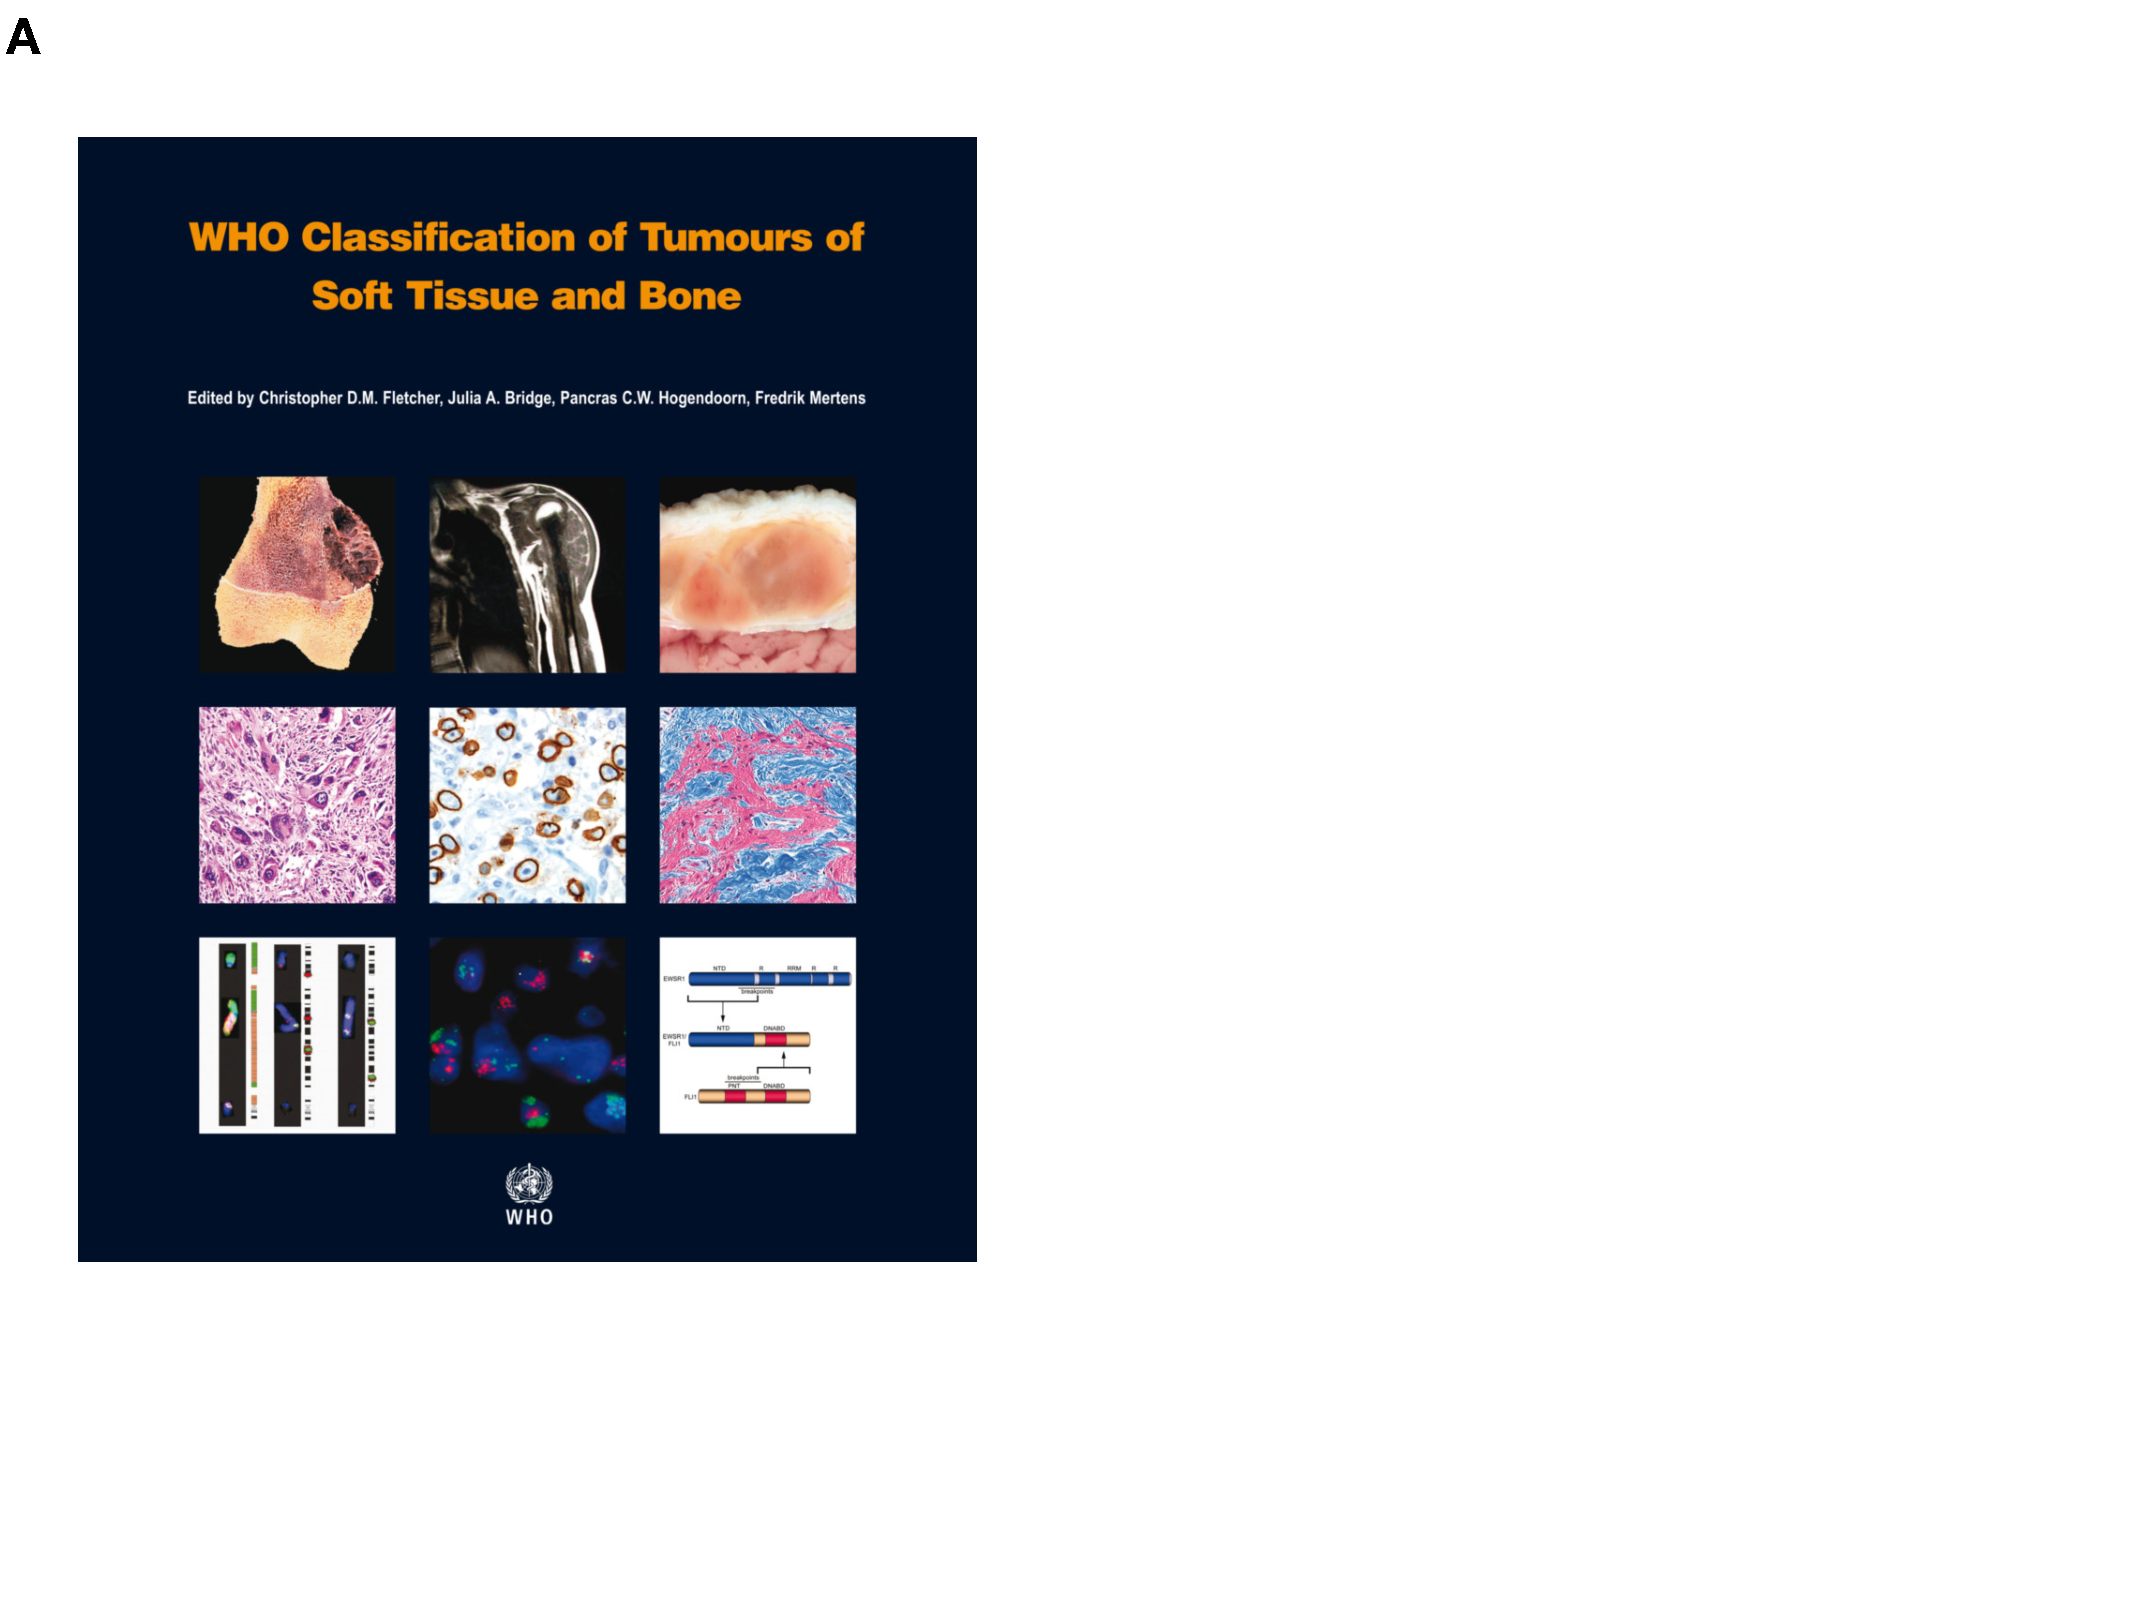
\includegraphics[height=6.75cm]{figures/intro/intro_context_1_2.pdf}\\
	\tiny{\textbf{A) } WHO classification book.}
		\onslide<2>\center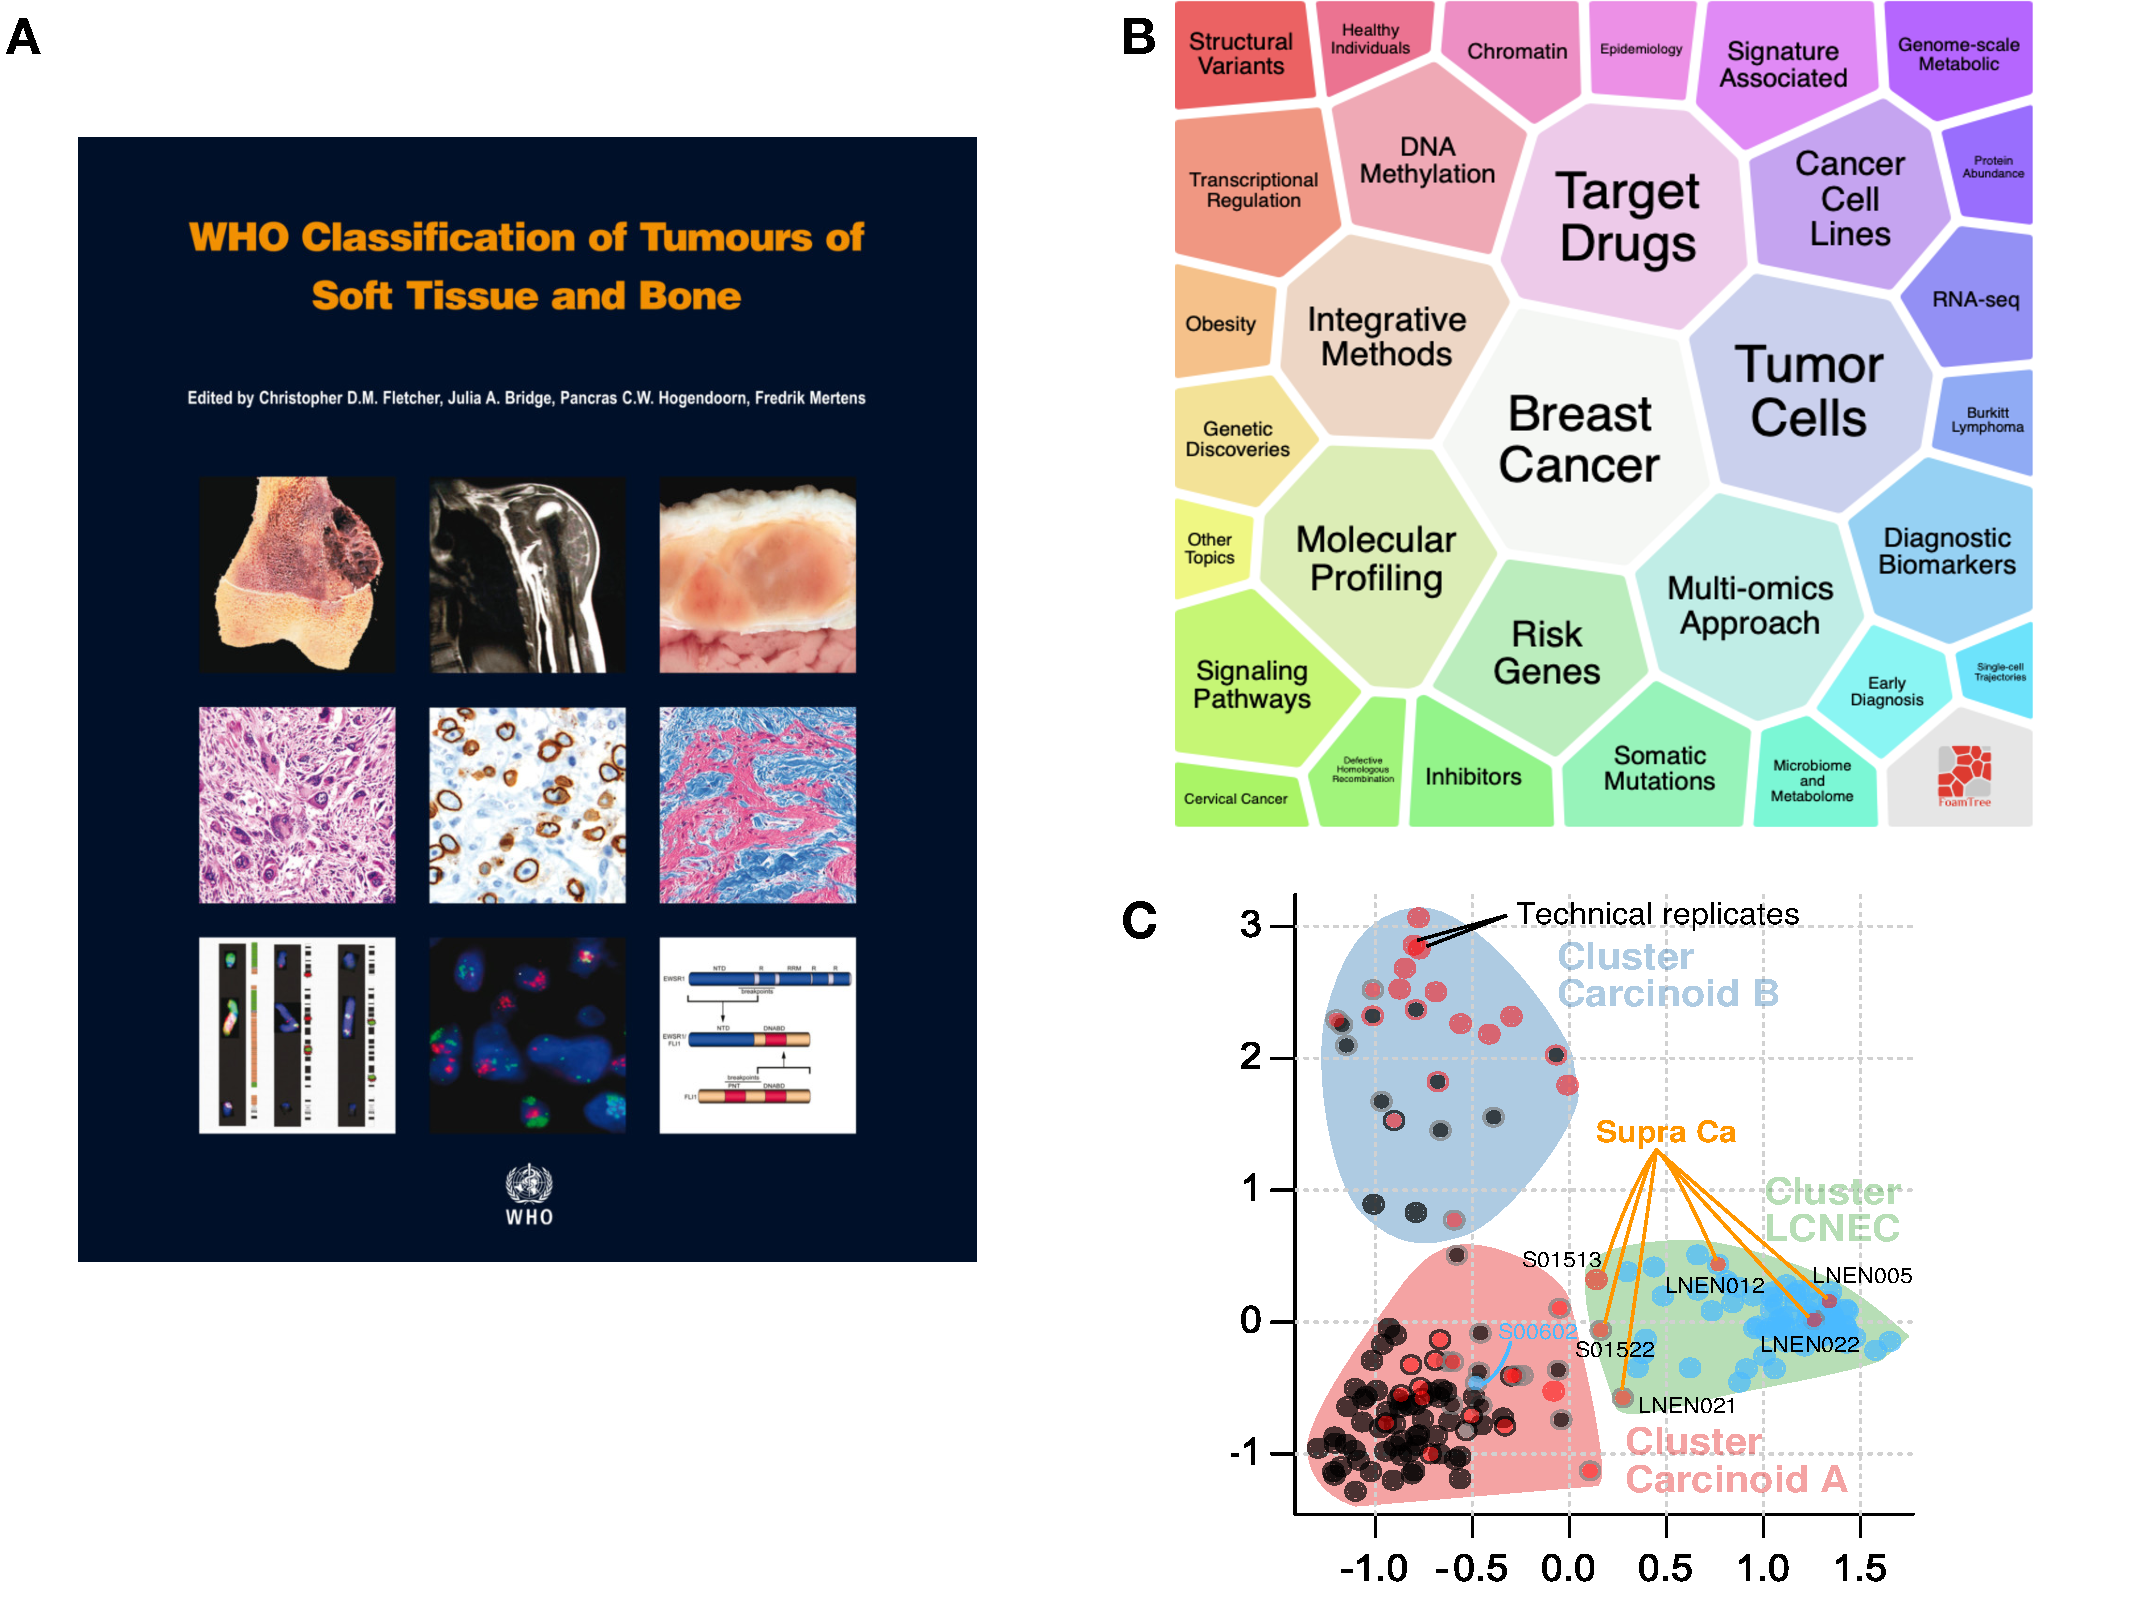
\includegraphics[height=6.75cm]{figures/intro/intro_context_2_2.pdf}\\
			\tiny{	\textbf{A) } WHO classification book. \textbf{B) } FoamTree with the words genomic and cancer. \\
			\textbf{C) } MOFA on LNEN samples \cite{alcala2019integrative}} 
	\end{overprint}
\end{figure}

  \begin{flushright}
\color{IARCdblue}{  \scriptsize{\insertframenumber / \inserttotalframenumber}} \hspace*{2mm}
  \end{flushright}

\end{frame}

%%%%%%%%%%%%%%%%%%%%%%%%%%
\section{Introduction : Dimensionality reduction to summarize data}
\begin{frame}
\vspace*{-1cm}



    \begin{overprint}
    \onslide<1>
\begin{columns}[t]
  \begin{column}{0.75\linewidth}
  \vspace*{-0.4cm}

  \begin{figure}
\centering
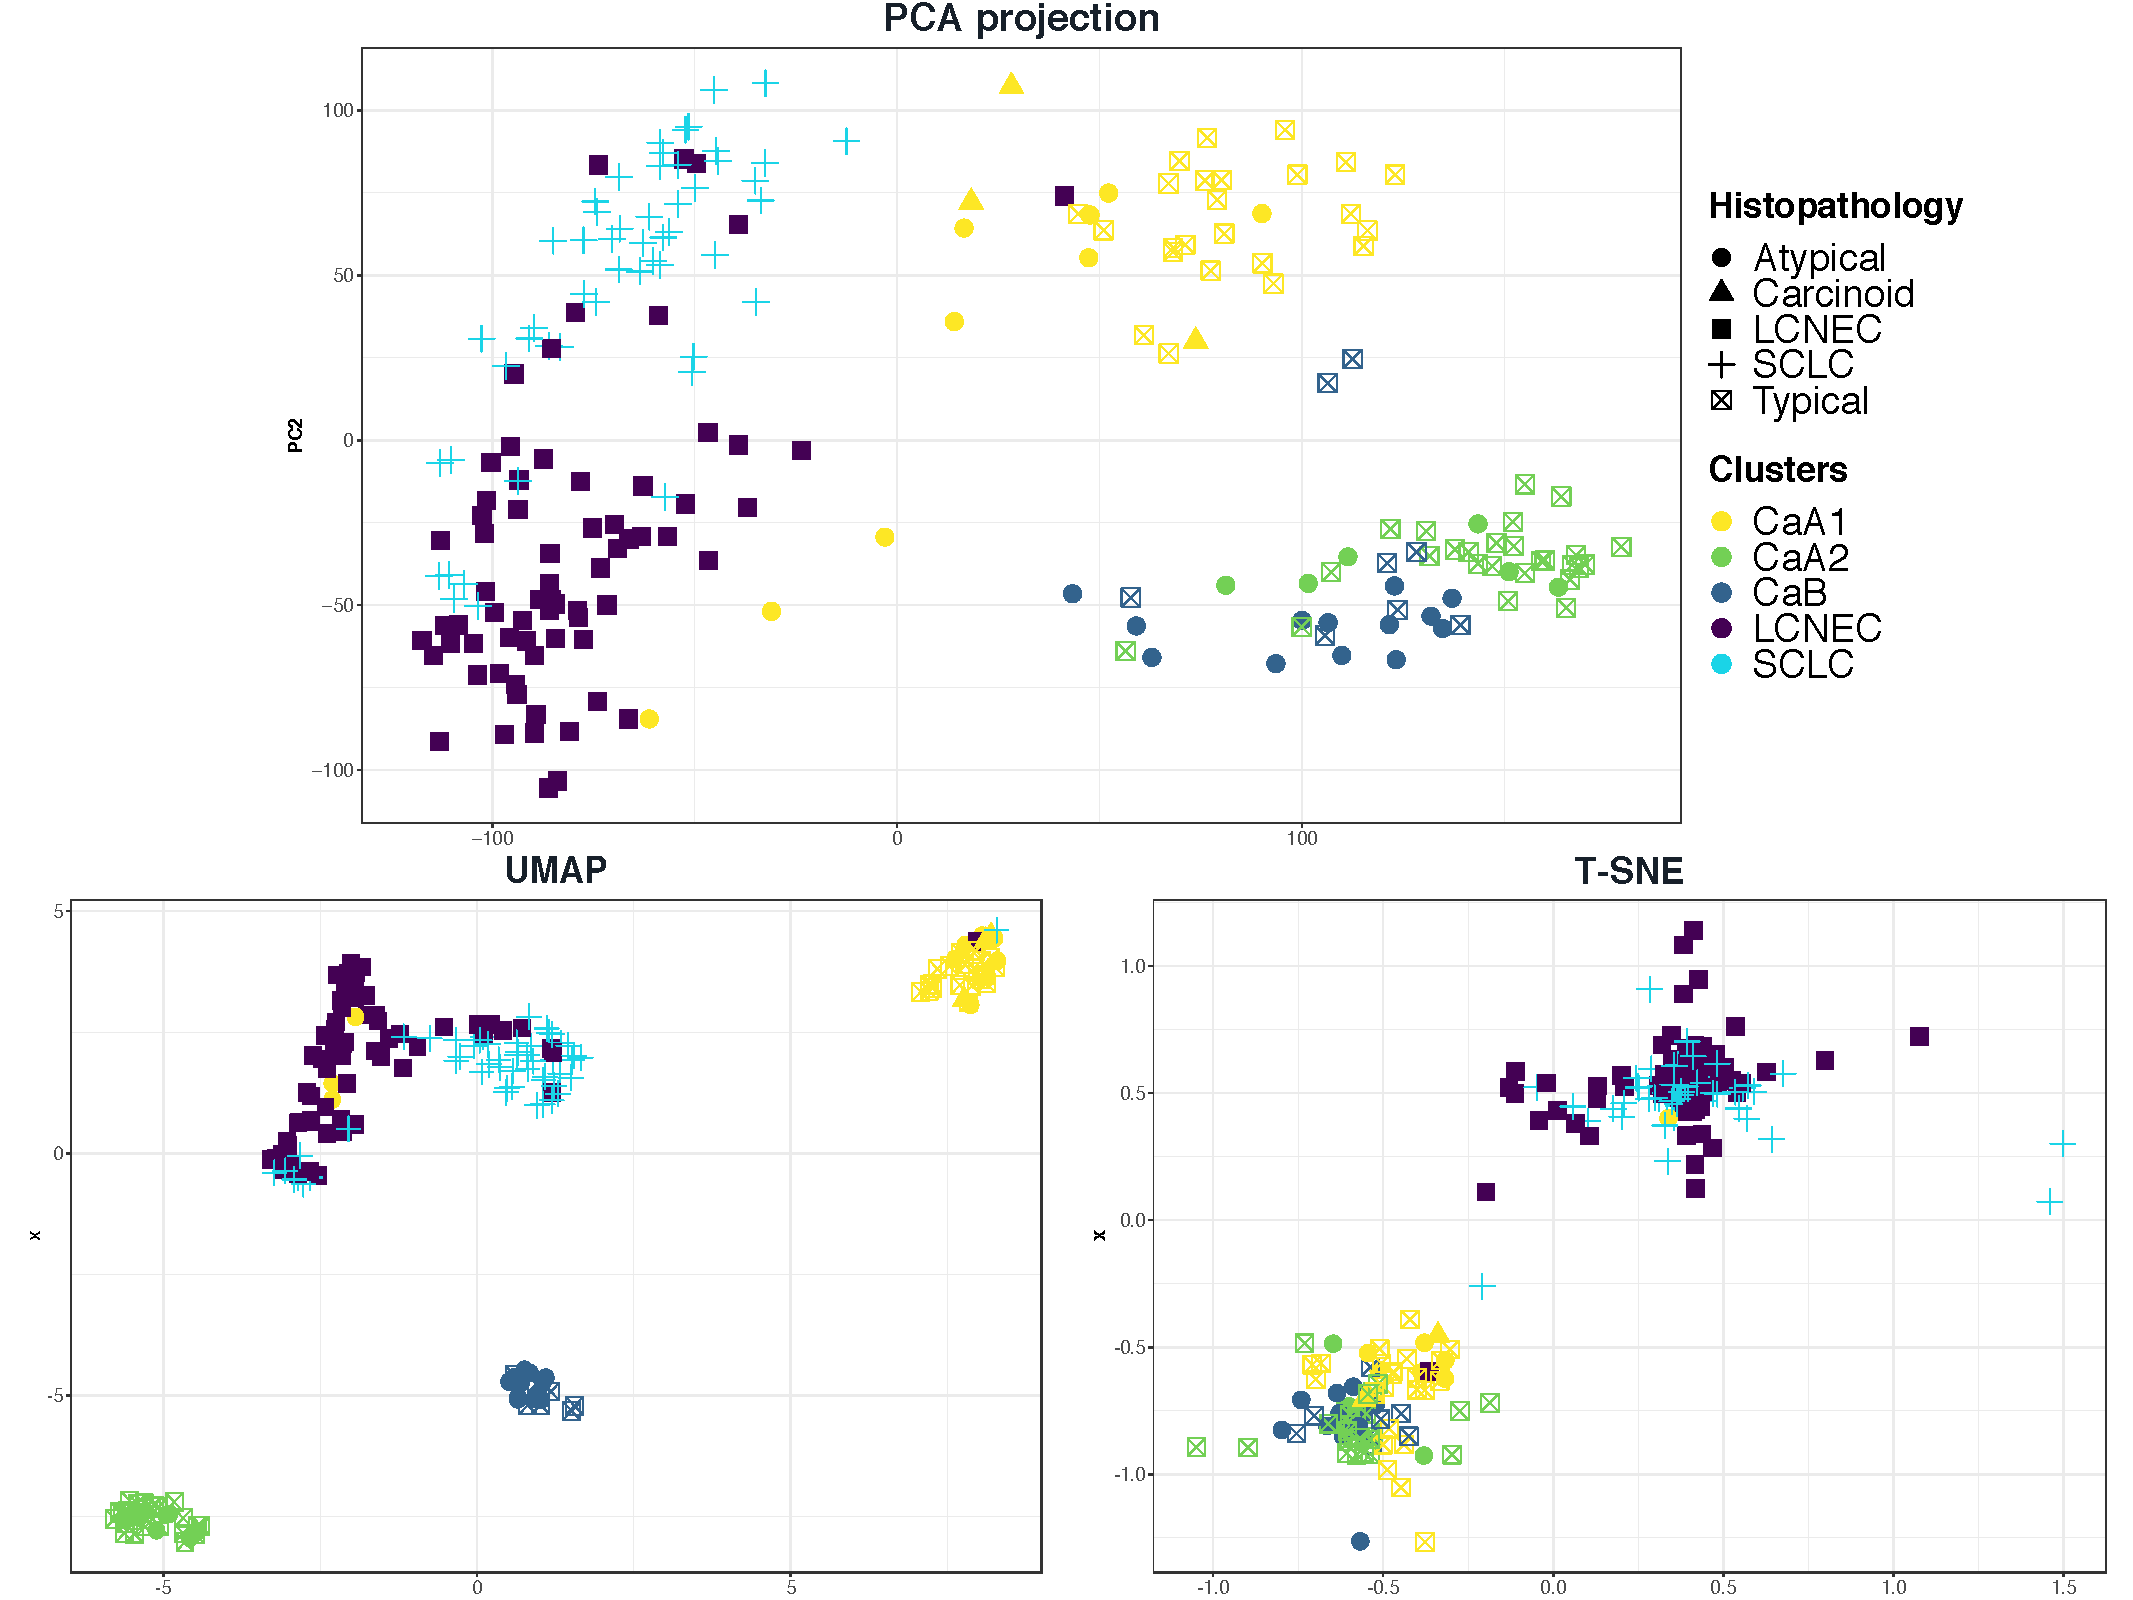
\includegraphics[height=0.75\linewidth]{figures/intro/RD3.pdf}
  \end{figure}
  \end{column}
  \hspace{-0.7cm}
  \begin{column}{0.25\linewidth}
  \end{column}
 \end{columns} 
 
    \onslide<2>
    \begin{columns}[c]
  \begin{column}{0.75\linewidth}
    \vspace*{-0.4cm}
  \begin{figure}
\centering
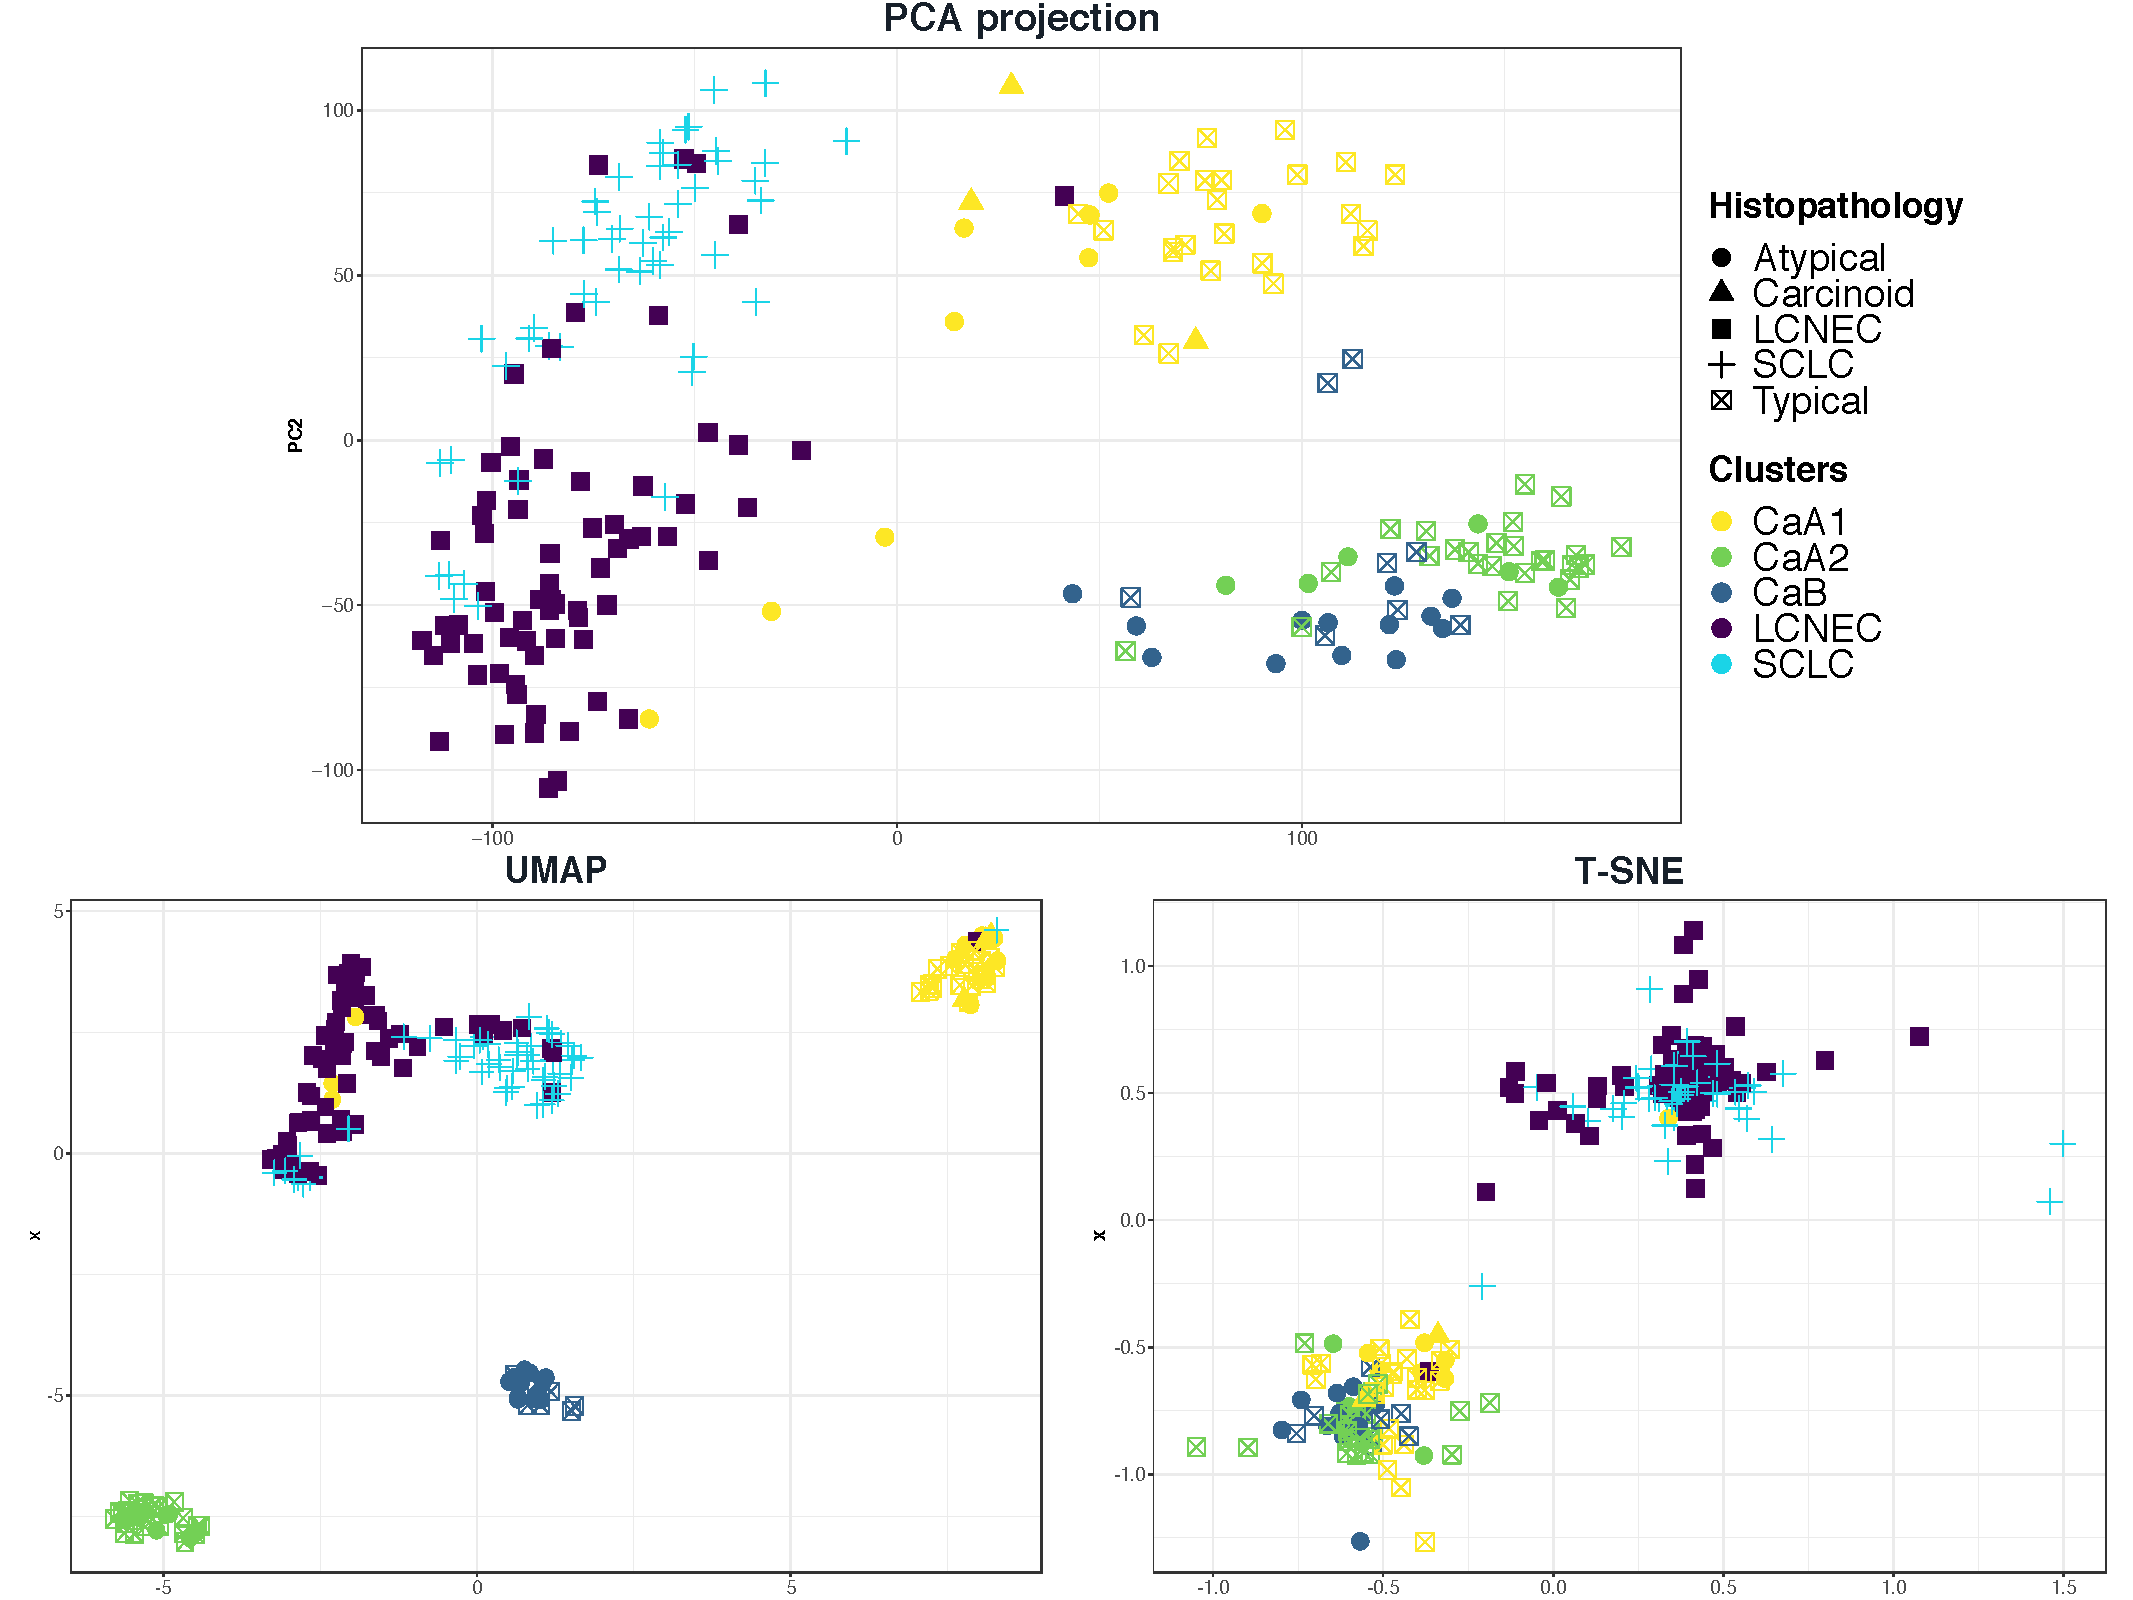
\includegraphics[height=0.75\linewidth]{figures/intro/RD3.pdf}
  \end{figure}
  \end{column}
  \hspace{-0.7cm}

  \begin{column}{0.25\linewidth}

  \hskip8pt 
    \textcolor{IARCblue}{Problematics : }
  \begin{itemize}
        \item Omics data interpretation
      \item Hypothesis generation 
  \end{itemize}
  \end{column}
 \end{columns} 
  
    \onslide<3>
        
    \begin{columns}[c]
  \begin{column}{0.75\linewidth}
    \vspace*{-0.4cm}
  \begin{figure}
\centering
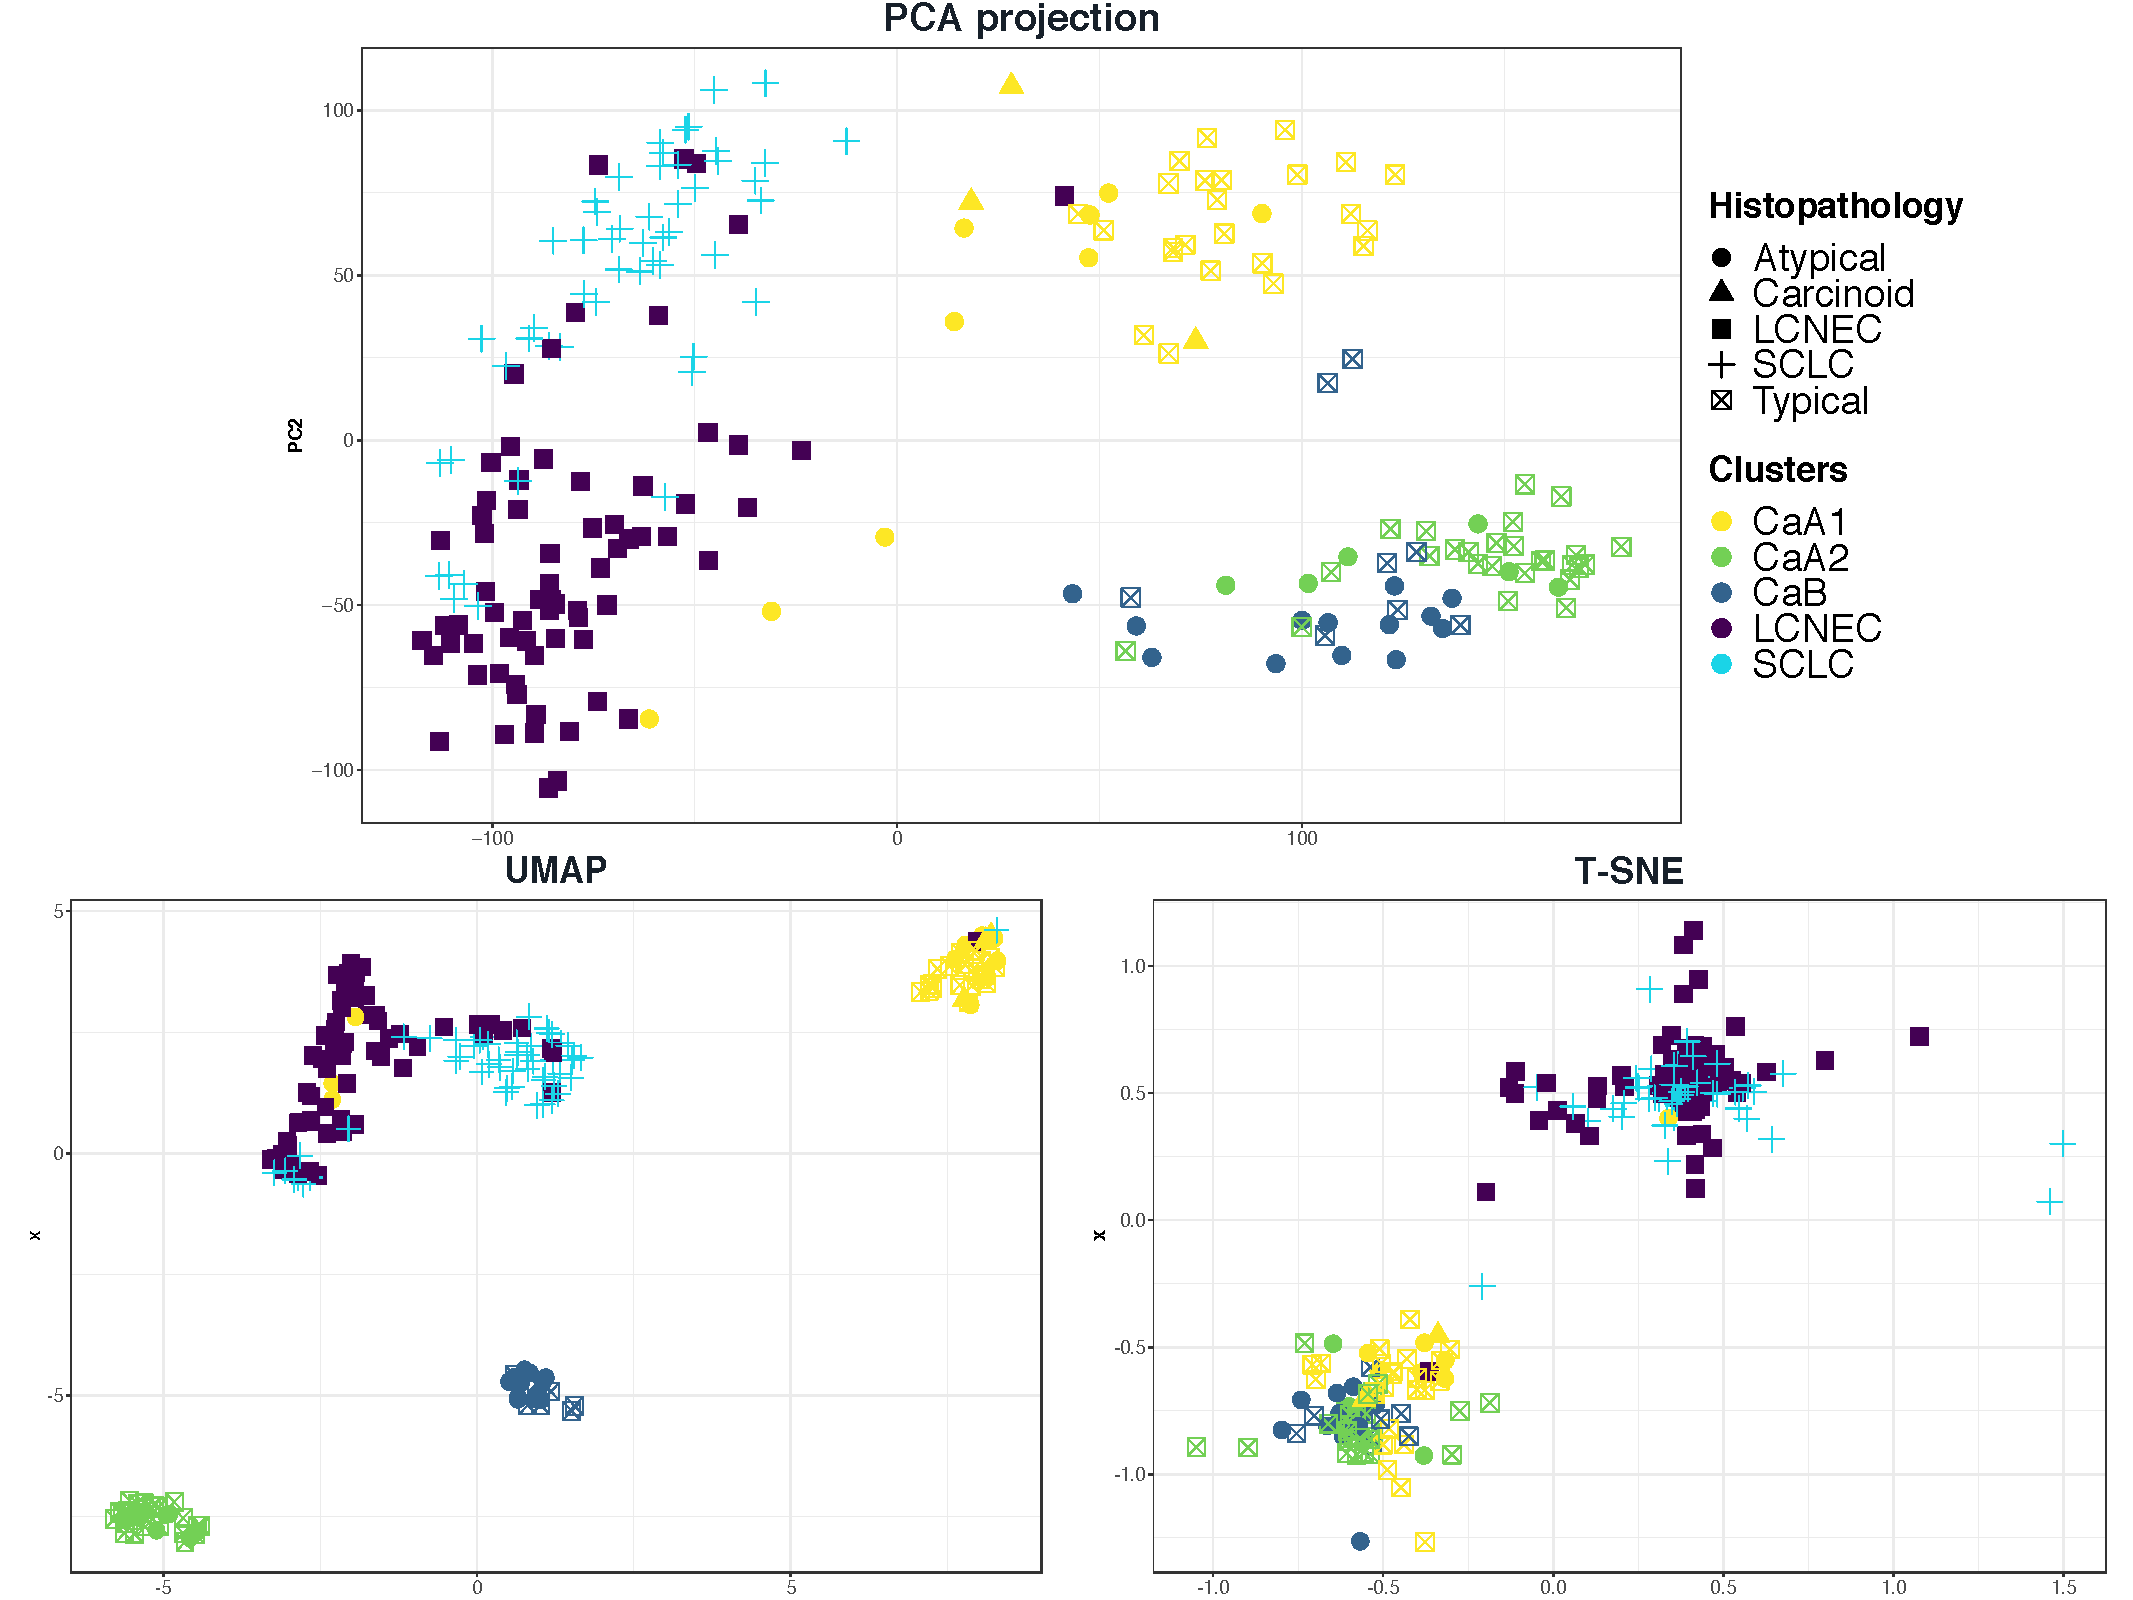
\includegraphics[height=0.75\linewidth]{figures/intro/RD3.pdf}
  \end{figure}
  \end{column}
  \hspace{-0.7cm}
  \begin{column}{0.25\linewidth}

  \hskip8pt 
    \textcolor{IARCblue}{Problematics : }
  \begin{itemize}
        \item Omics data interpretation
      \item Hypothesis generation 
      \item Comparatives metrics
      \item Clusters consistancy
  \end{itemize}
  \end{column}
 \end{columns} 
  
\end{overprint}


  \begin{flushright}
\color{IARCdblue}{ \scriptsize{\insertframenumber / \inserttotalframenumber}} \hspace*{2mm}
  \end{flushright}

\end{frame}


%%%%%%%%%%%%%% Methods  %%%%%%%%%%%%%%%%%%%%%%%%%%%%%%%%%%%%%%%%%%%%%


\section{Methods : Dimensionality reduction (DR) methods}
\begin{frame}
\vspace*{-1.4cm}

    \begin{overprint}
    \onslide<1>
\begin{columns}[c]
  \begin{column}{0.5\linewidth}
  \begin{figure}
\centering
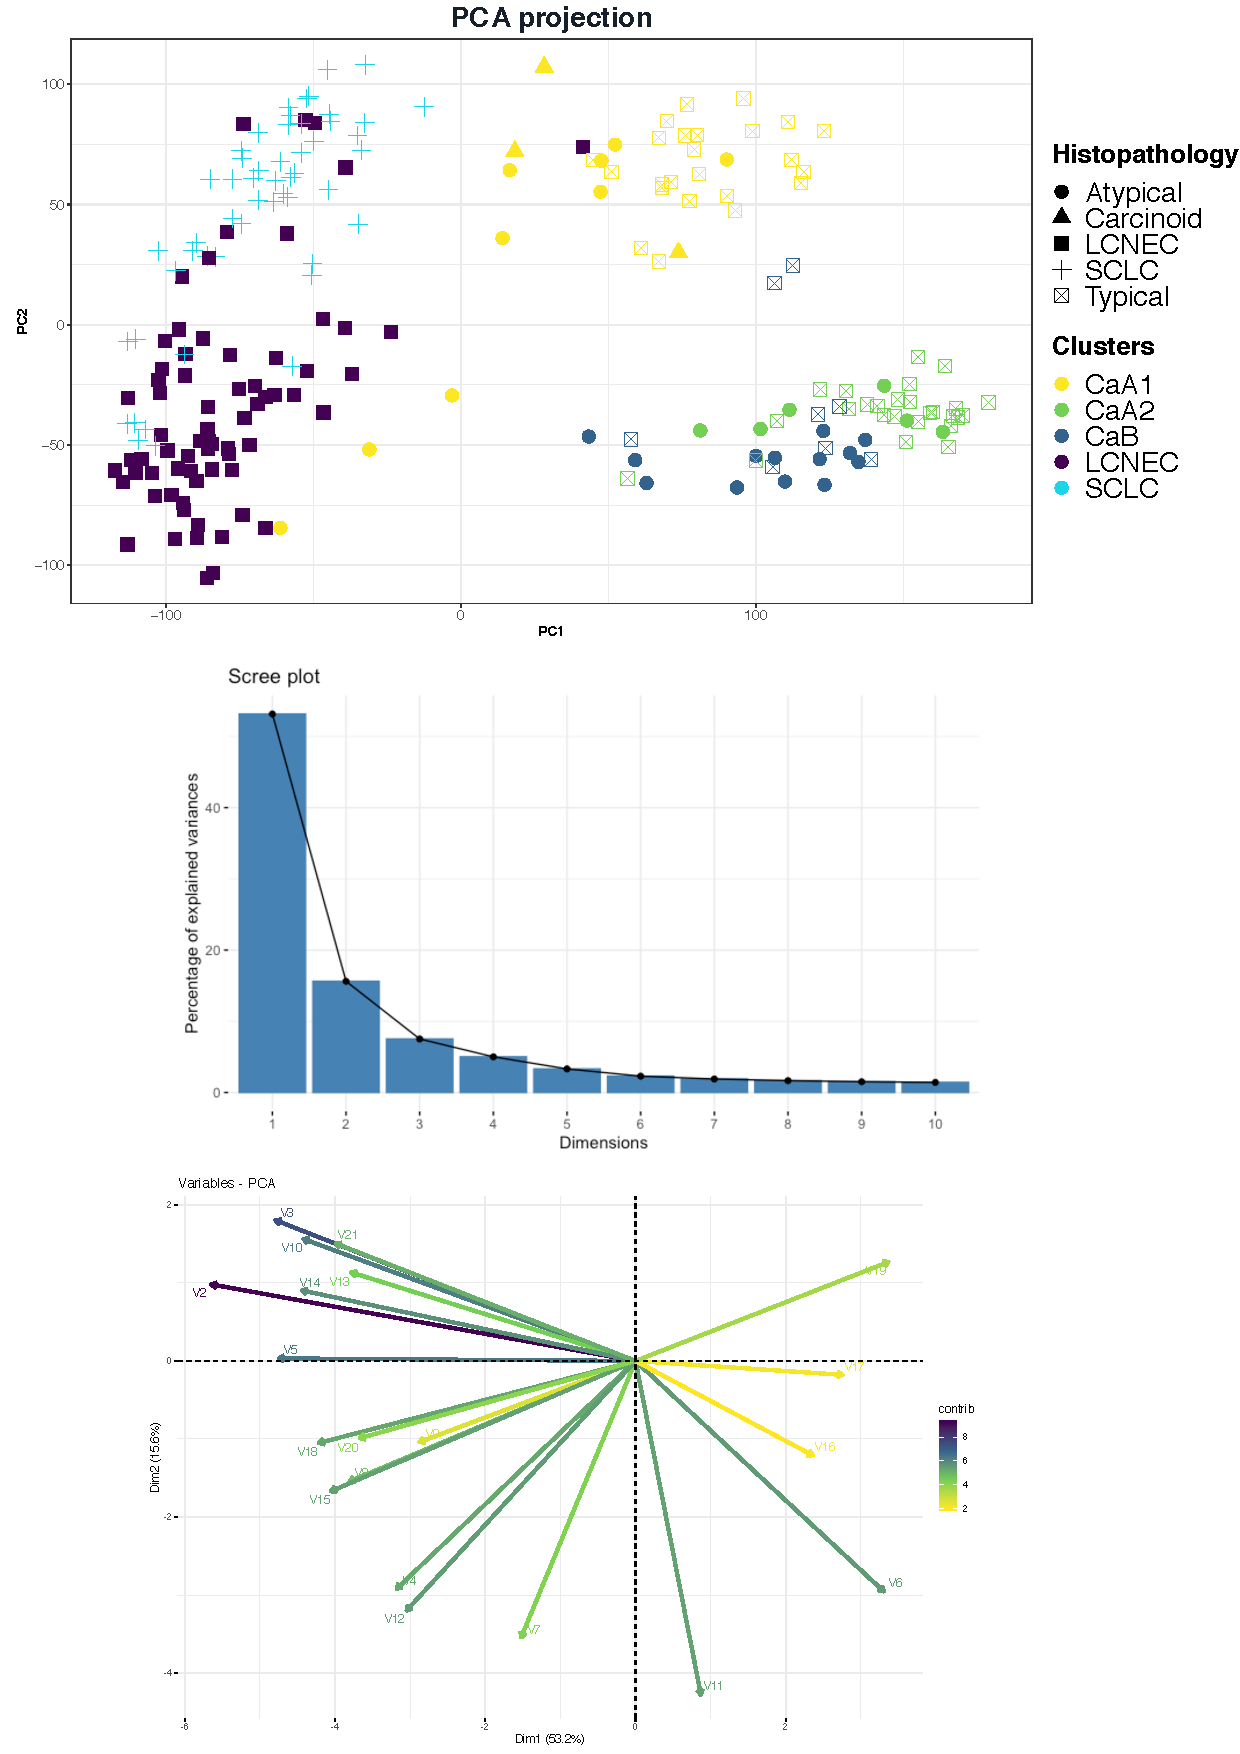
\includegraphics[height=7cm]{figures/methods/pca-methods2.pdf}
  \end{figure}
  \end{column}
  \hspace{-0.7cm}
  \begin{column}{0.5\linewidth}
  \end{column}
 \end{columns} 
 
  
     \onslide<2>
\begin{columns}[c]
  \begin{column}{0.5\linewidth}
  \begin{figure}
\centering
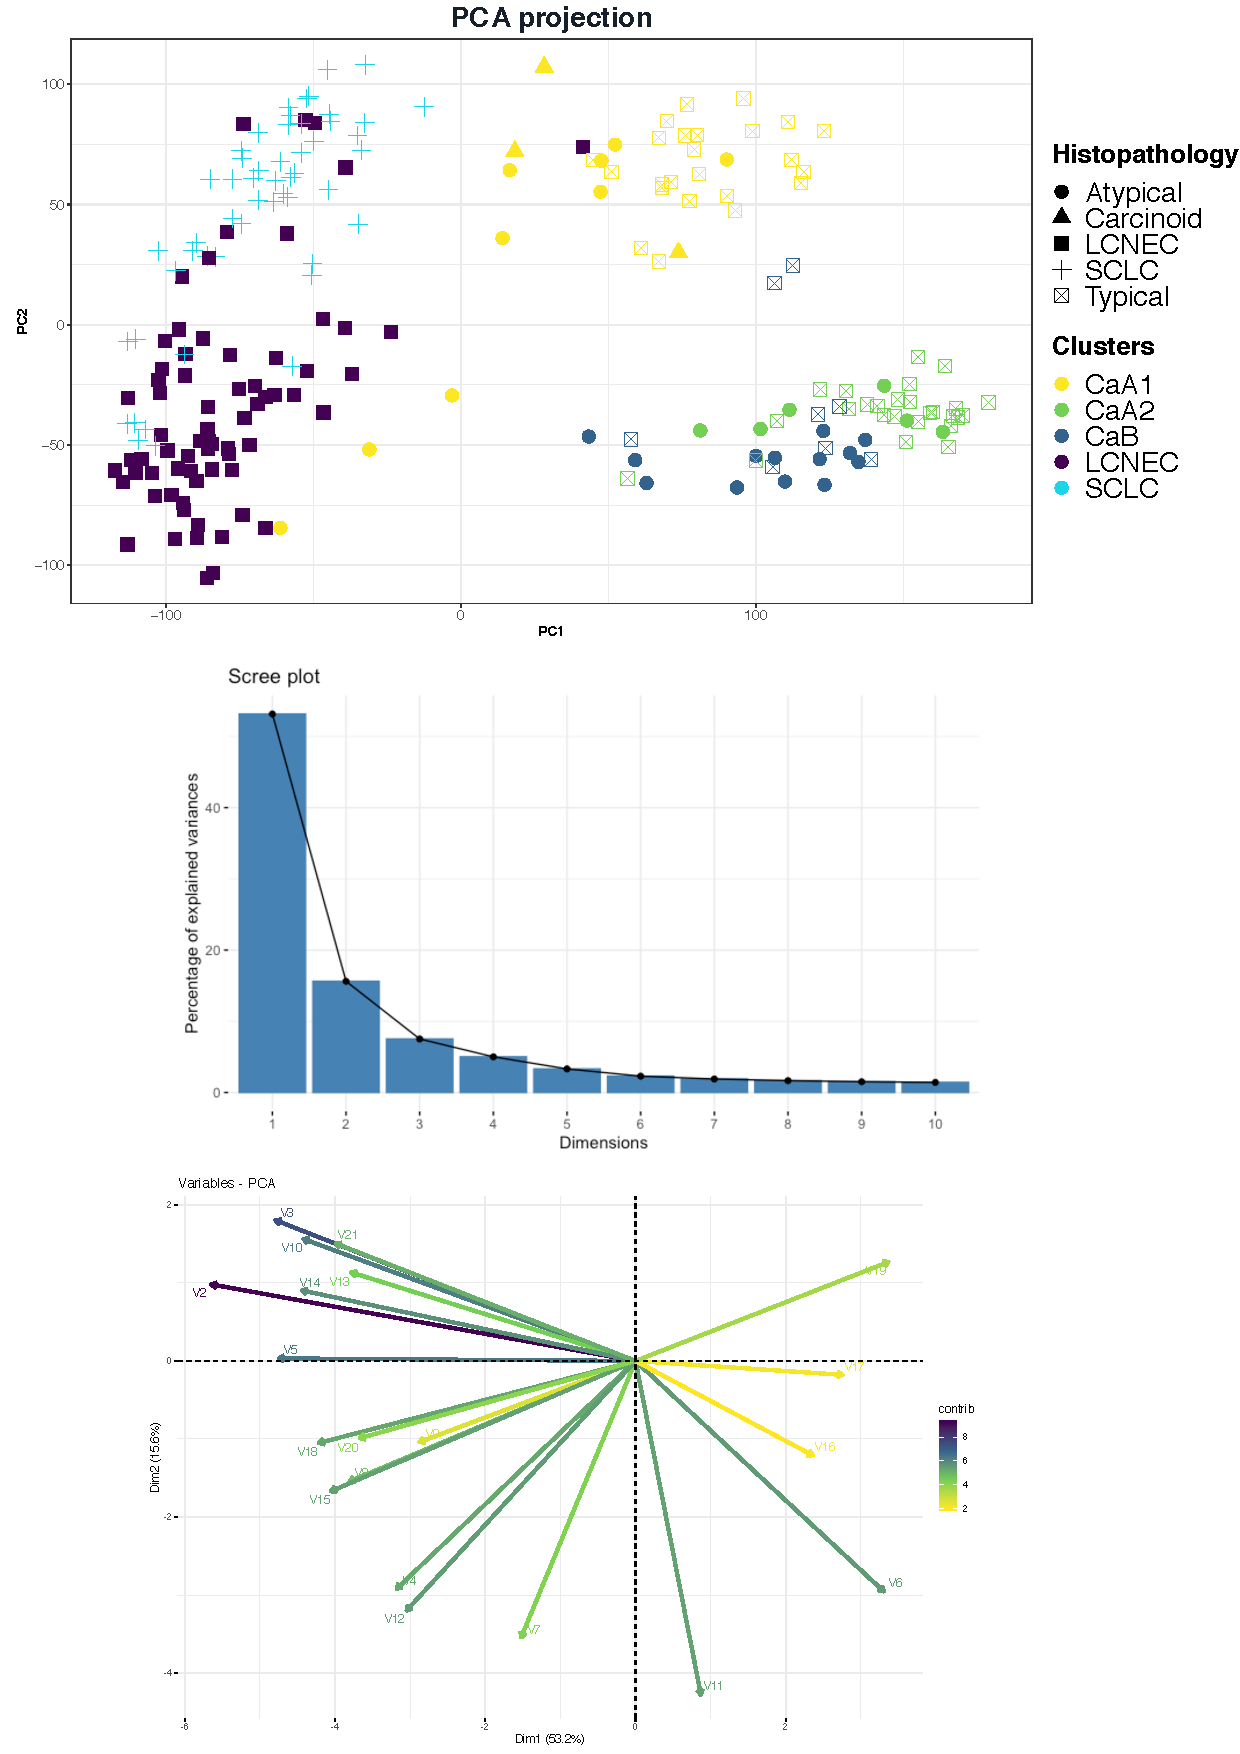
\includegraphics[height=7cm]{figures/methods/pca-methods2.pdf}
  \end{figure}
  \end{column}

  \begin{column}{0.5\linewidth}
   \begin{figure}
\centering
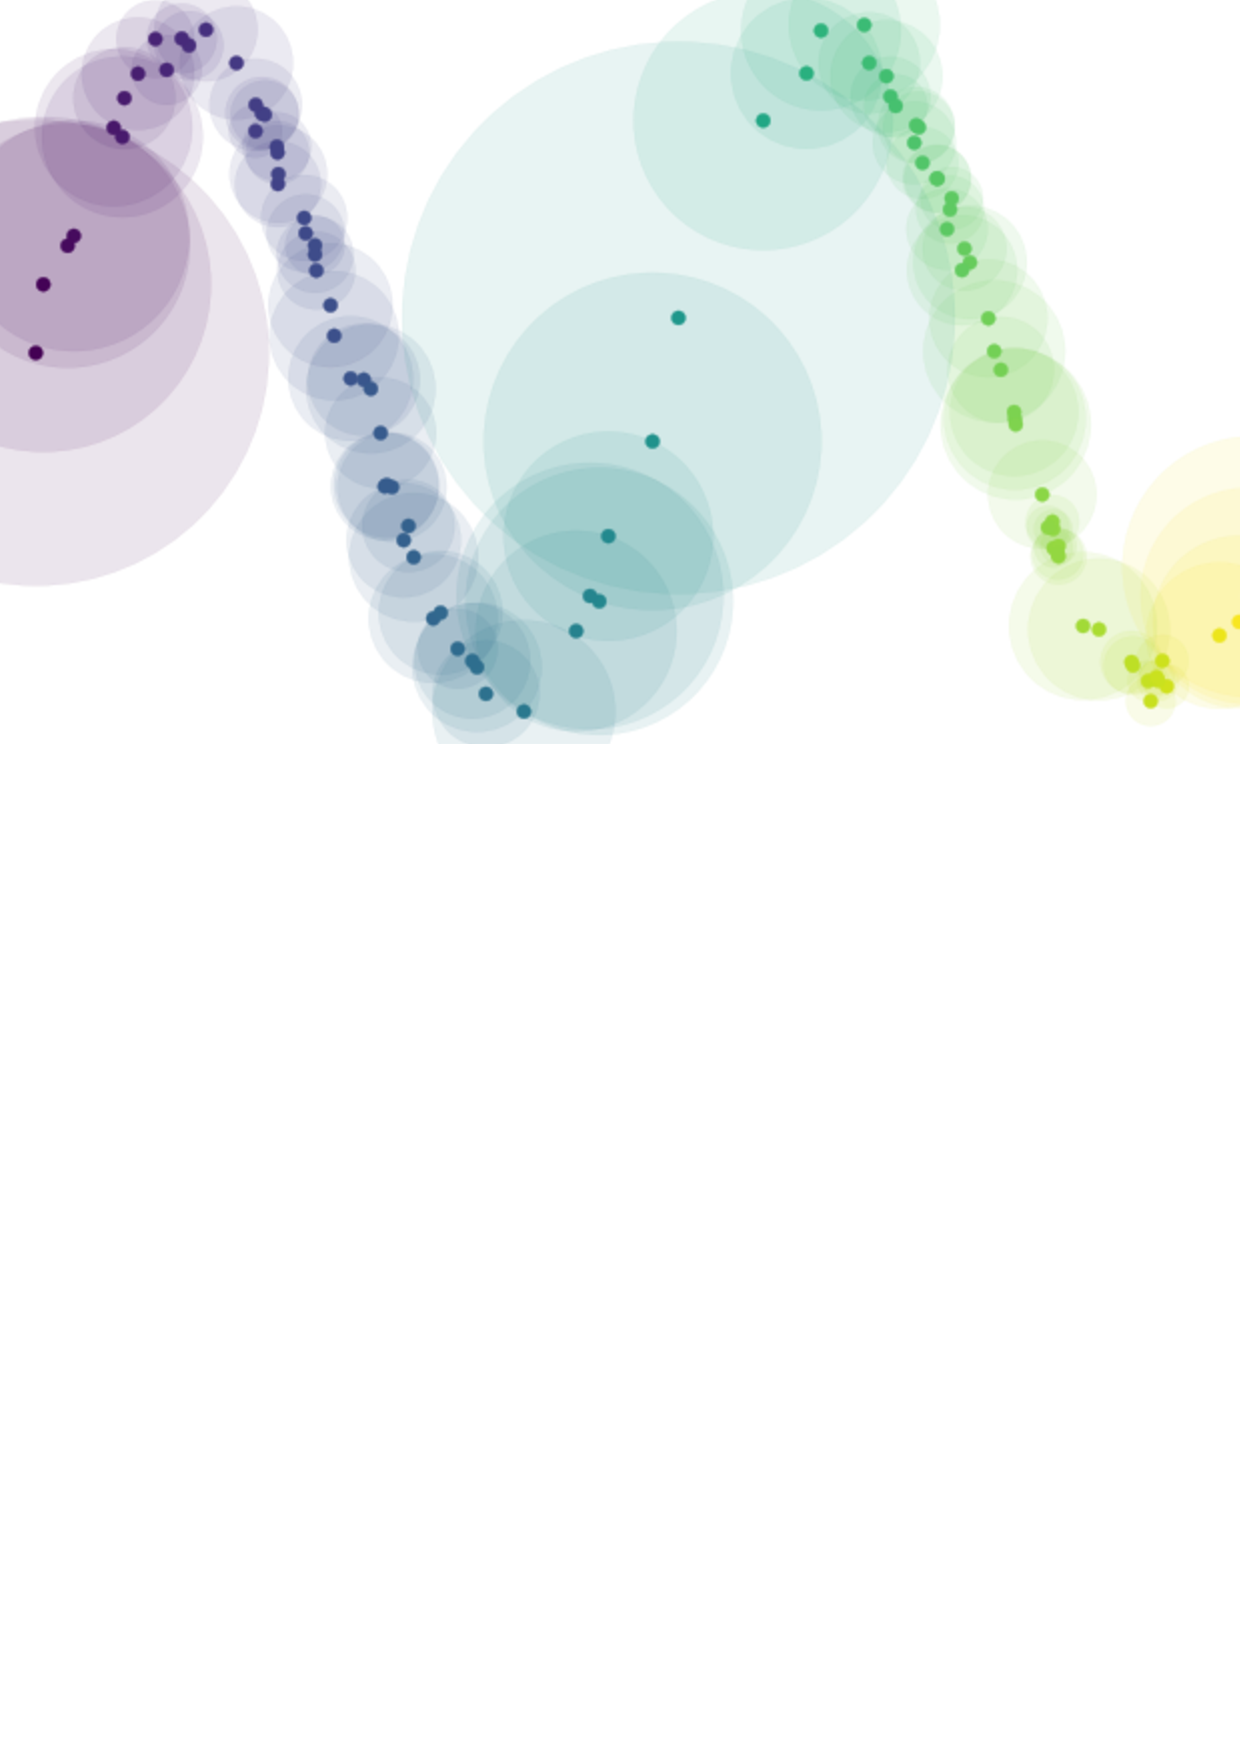
\includegraphics[height=7cm]{figures/methods/how_umap_works_local_metric_open_cover.pdf}
  \end{figure}
  \end{column}
 \end{columns} 
  
 
  
     \onslide<3>
\begin{columns}[c]
  \begin{column}{0.5\linewidth}
  \begin{figure}
\centering
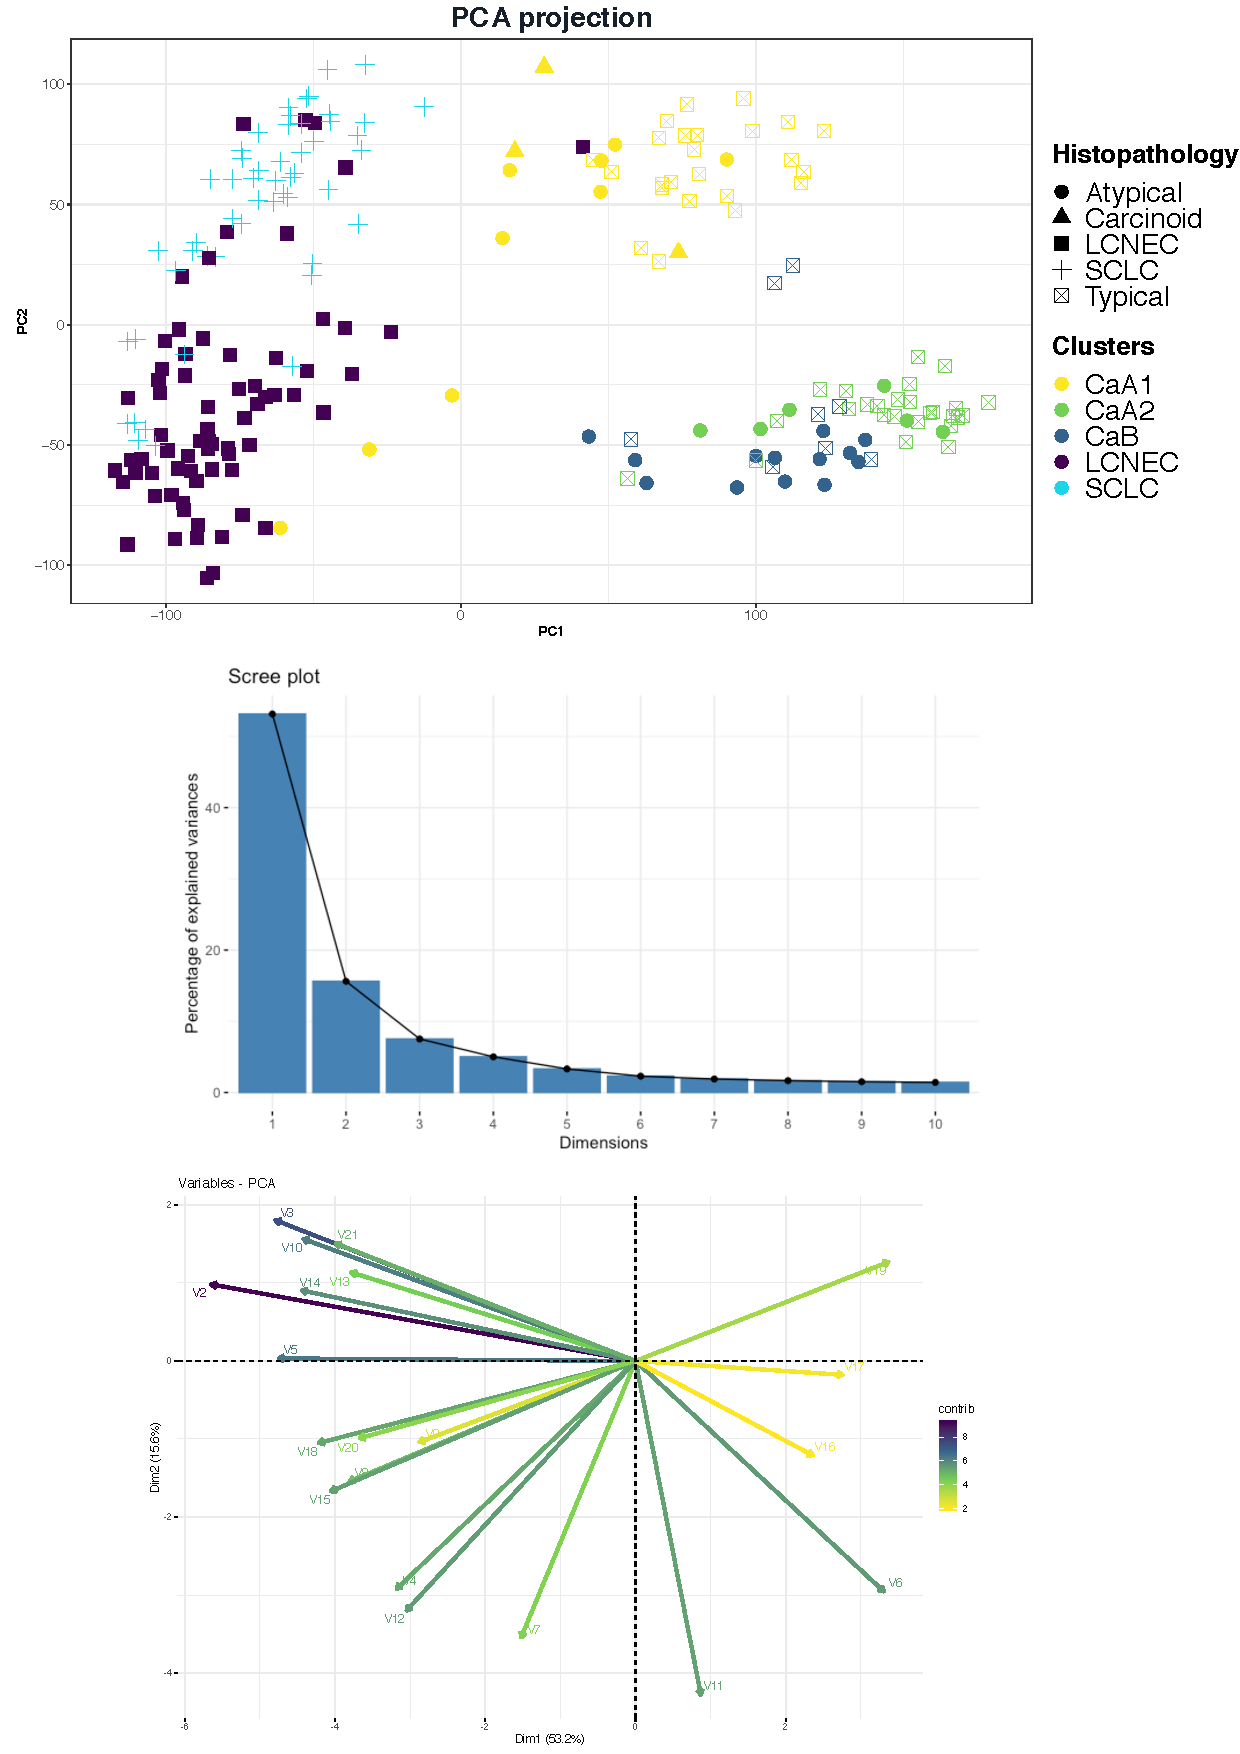
\includegraphics[height=7cm]{figures/methods/pca-methods2.pdf}
  \end{figure}
  \end{column}

  \begin{column}{0.5\linewidth}
   \begin{figure}
\centering
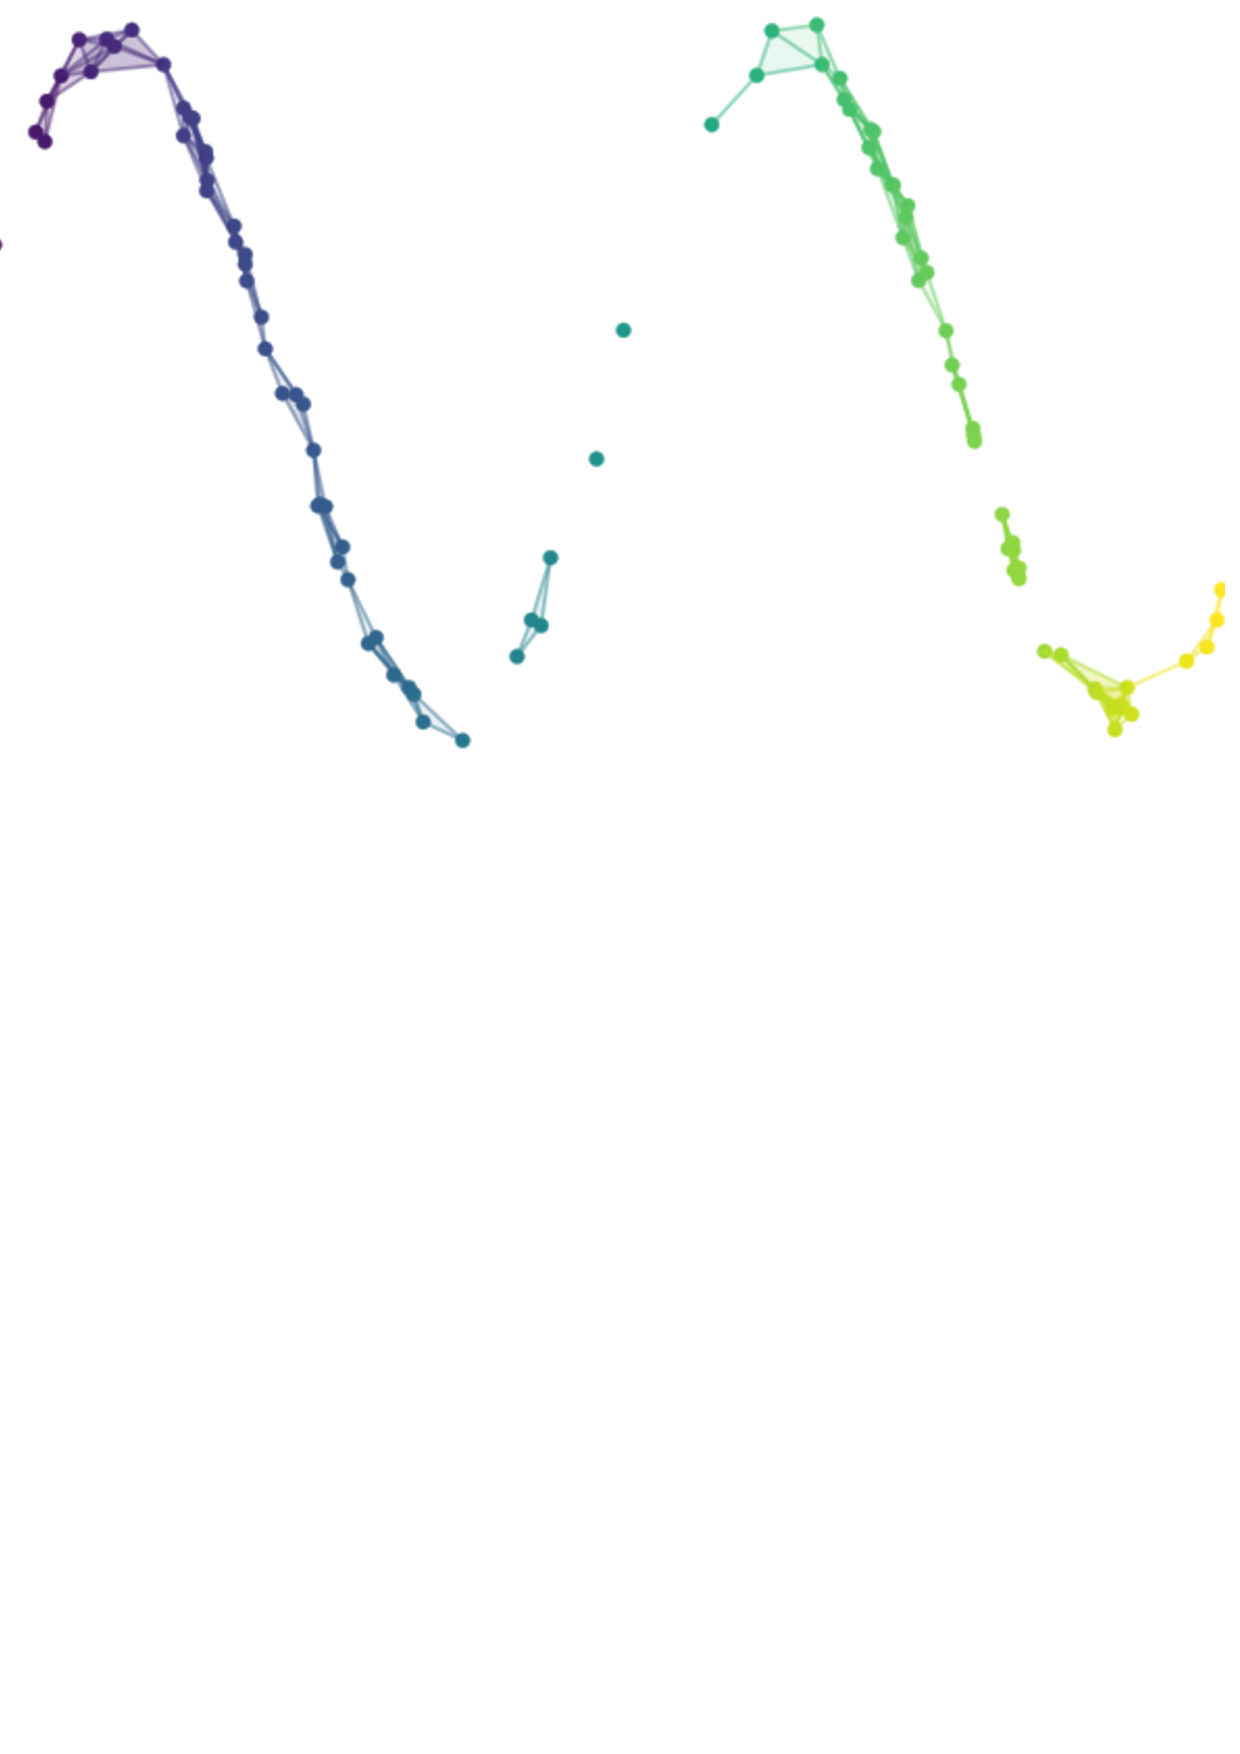
\includegraphics[height=7cm]{figures/methods/how_umap_works_basic_graph.pdf}
  \end{figure}
  \end{column}
 \end{columns}
 
 
      \onslide<4>
\begin{columns}[t]
  \begin{column}{0.5\linewidth}
  \begin{figure}
\centering
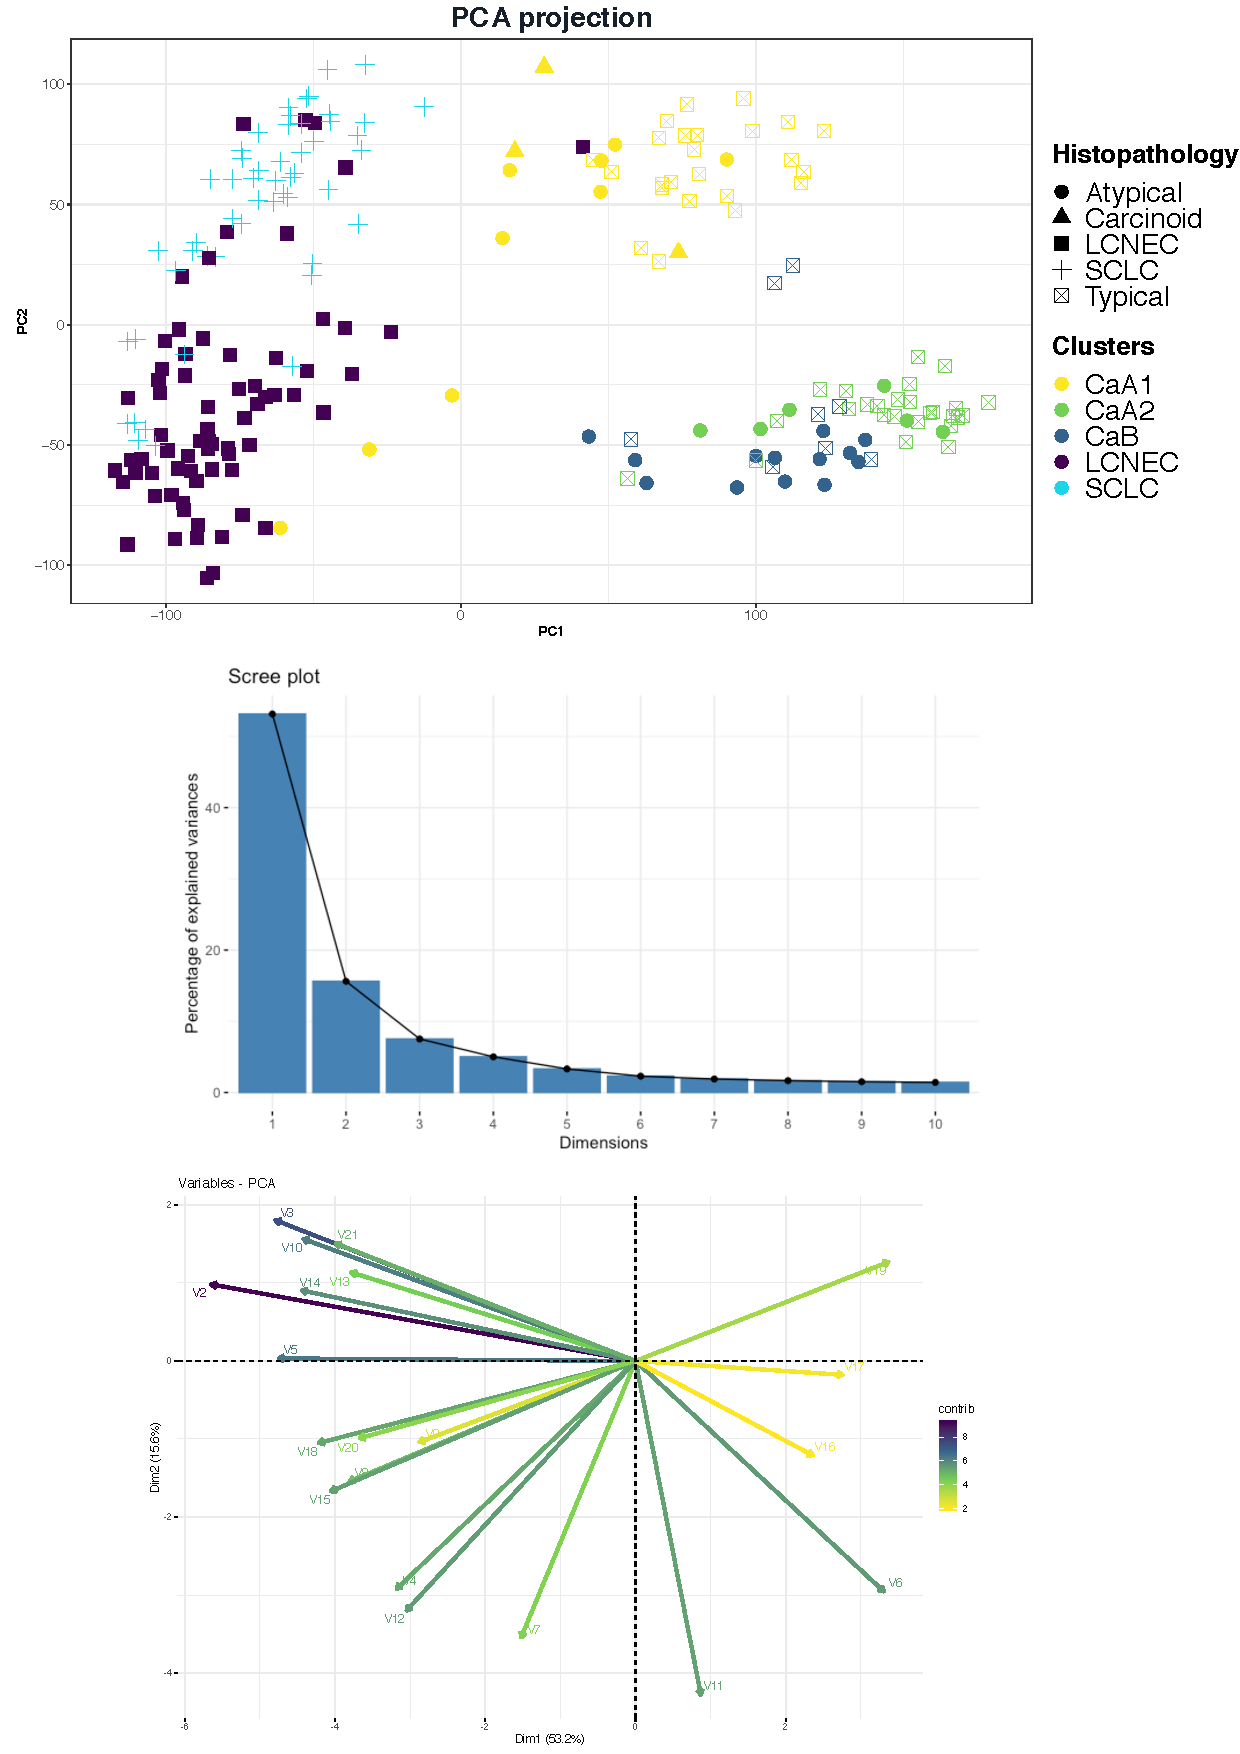
\includegraphics[height=7cm]{figures/methods/pca-methods2.pdf}
  \end{figure}
  \end{column}

  \begin{column}{0.5\linewidth}

     \begin{figure}
\centering
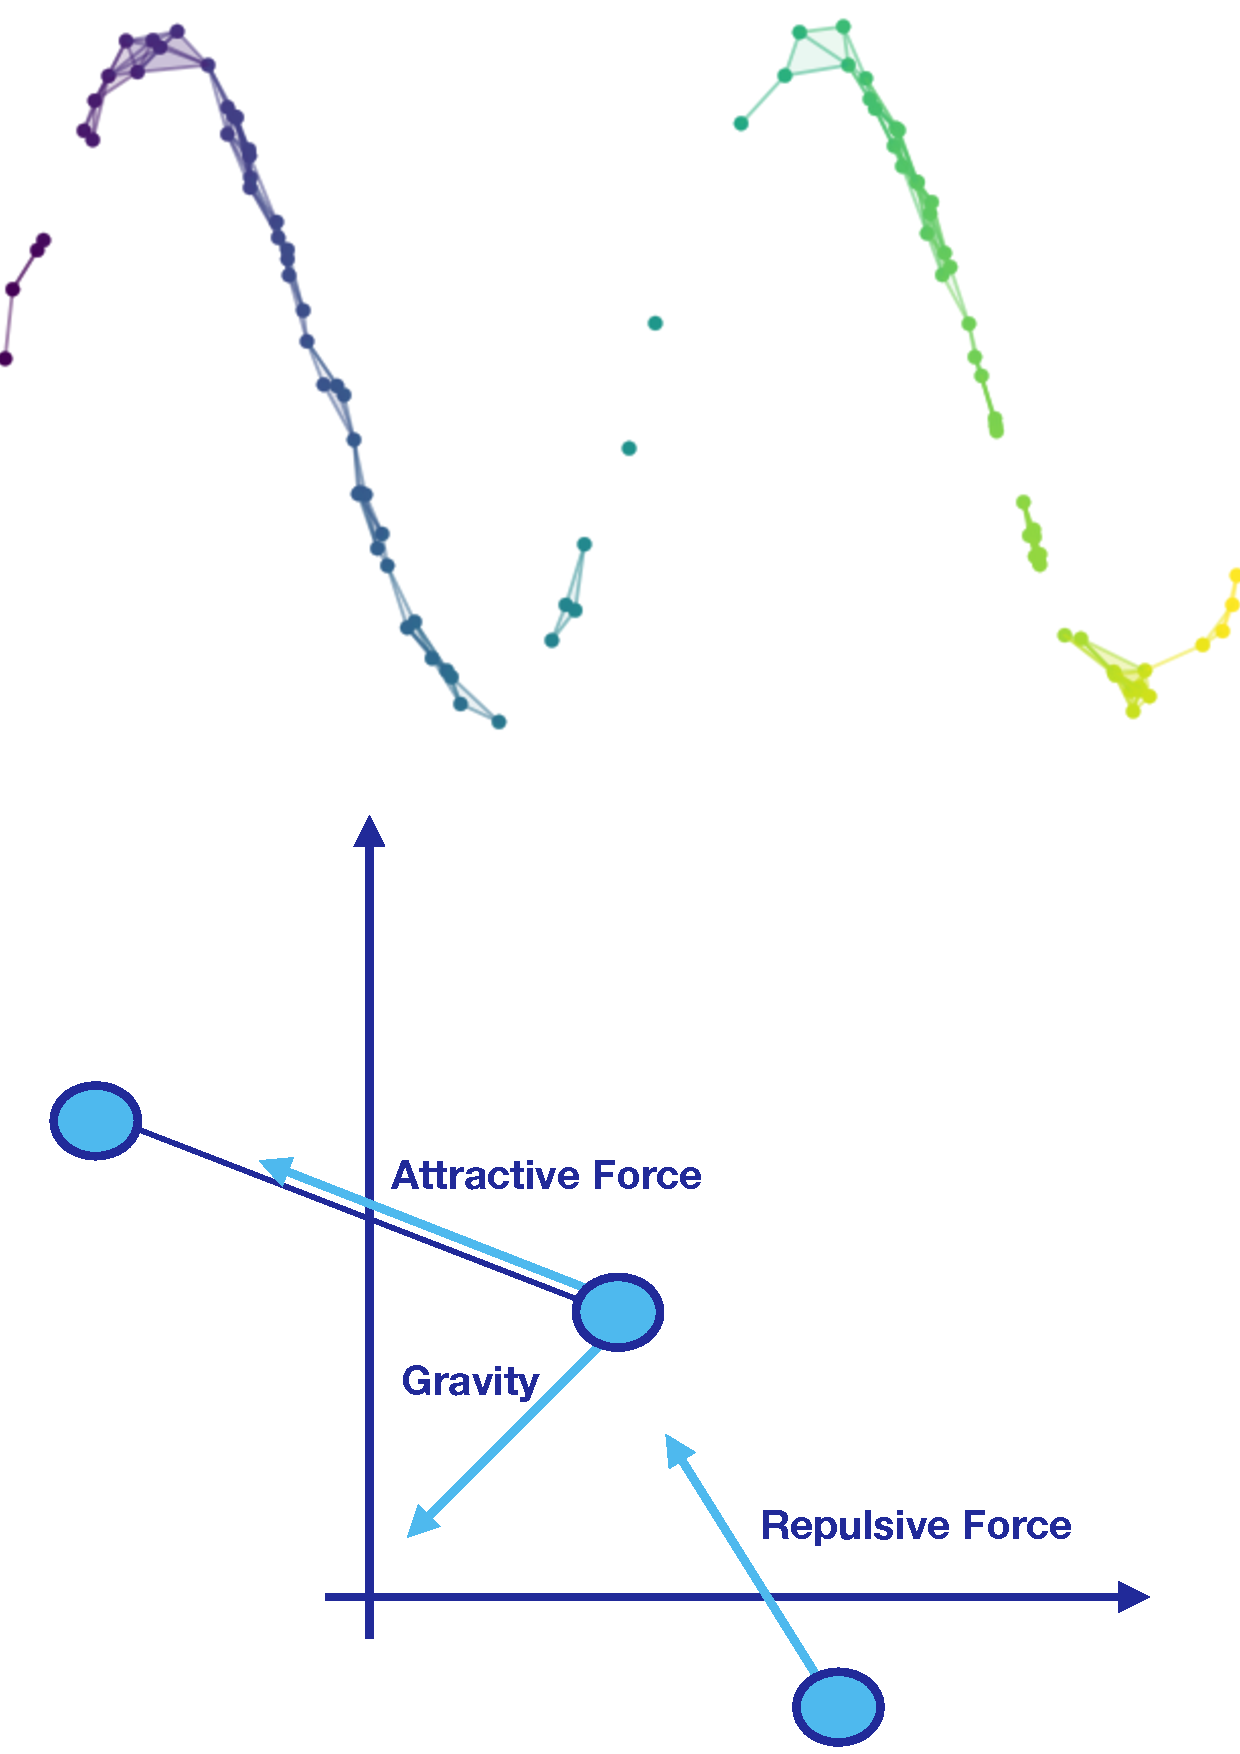
\includegraphics[height=7cm]{figures/methods/umap_forces.pdf}
  \end{figure}
    
  \end{column}
 \end{columns} 
  

  
  
\end{overprint}

  \begin{flushright}
\color{IARCdblue}{ \scriptsize{\insertframenumber / \inserttotalframenumber}} \hspace*{2mm}
  \end{flushright}

\end{frame}





%%%%%%%%%%%%%%%%%%%%%%%%%%%%%%%%%%% QUESTIONS %%%%%%%%%%%%%%%%
\section{Methods : Comparisons of DR methods}
\begin{frame}
\vspace*{-1cm}
    \begin{overprint}
    \onslide<1>
\begin{columns}[c]
  \begin{column}{0.55\linewidth}
 \begin{itemize}
     \item \textbf{Structure preservation : }\\
     \begin{itemize}
         \item Centrality 
         \item Neighborhood
     \end{itemize}
 \end{itemize}
  \end{column}

  \begin{column}{0.45\linewidth}
       \begin{figure}
\centering
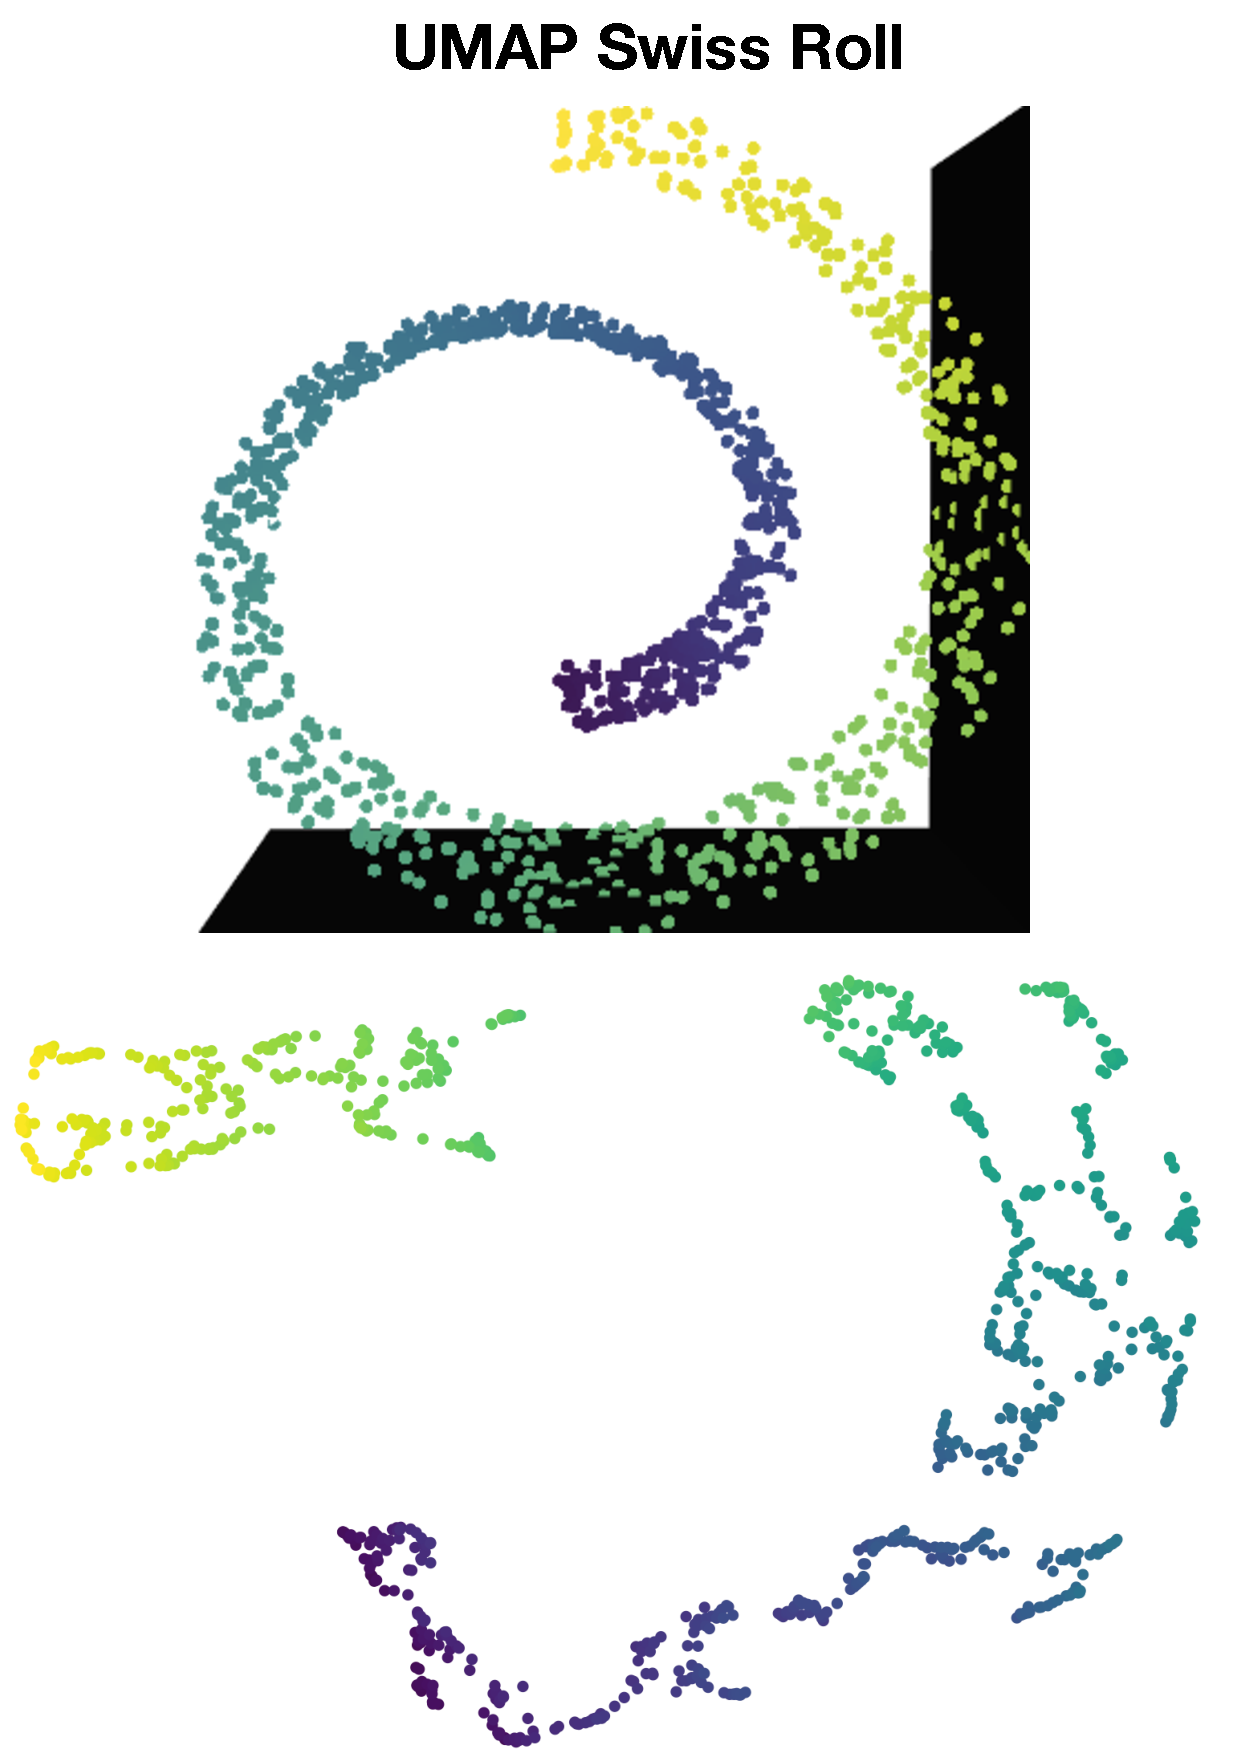
\includegraphics[height=7cm]{figures/methods/swiss_roll.pdf}
  \end{figure}
  \end{column}
 \end{columns} 
 
  
    \onslide<2>
\begin{columns}[c]
  \begin{column}{0.55\linewidth}
 \begin{itemize}
     \item \textbf{Structure preservation : }\\
     \begin{itemize}
         \item Centrality 
         \item Neighborhood
     \end{itemize}
 \end{itemize}
  \begin{itemize}
    \item   \textbf{Correlations' consistency : }\\
     \begin{itemize}
         \item Control of dataset's noise
         \item Highlighting key features 
     \end{itemize}
\end{itemize}
  \end{column}
  \begin{column}{0.45\linewidth}
       \begin{figure}
\centering
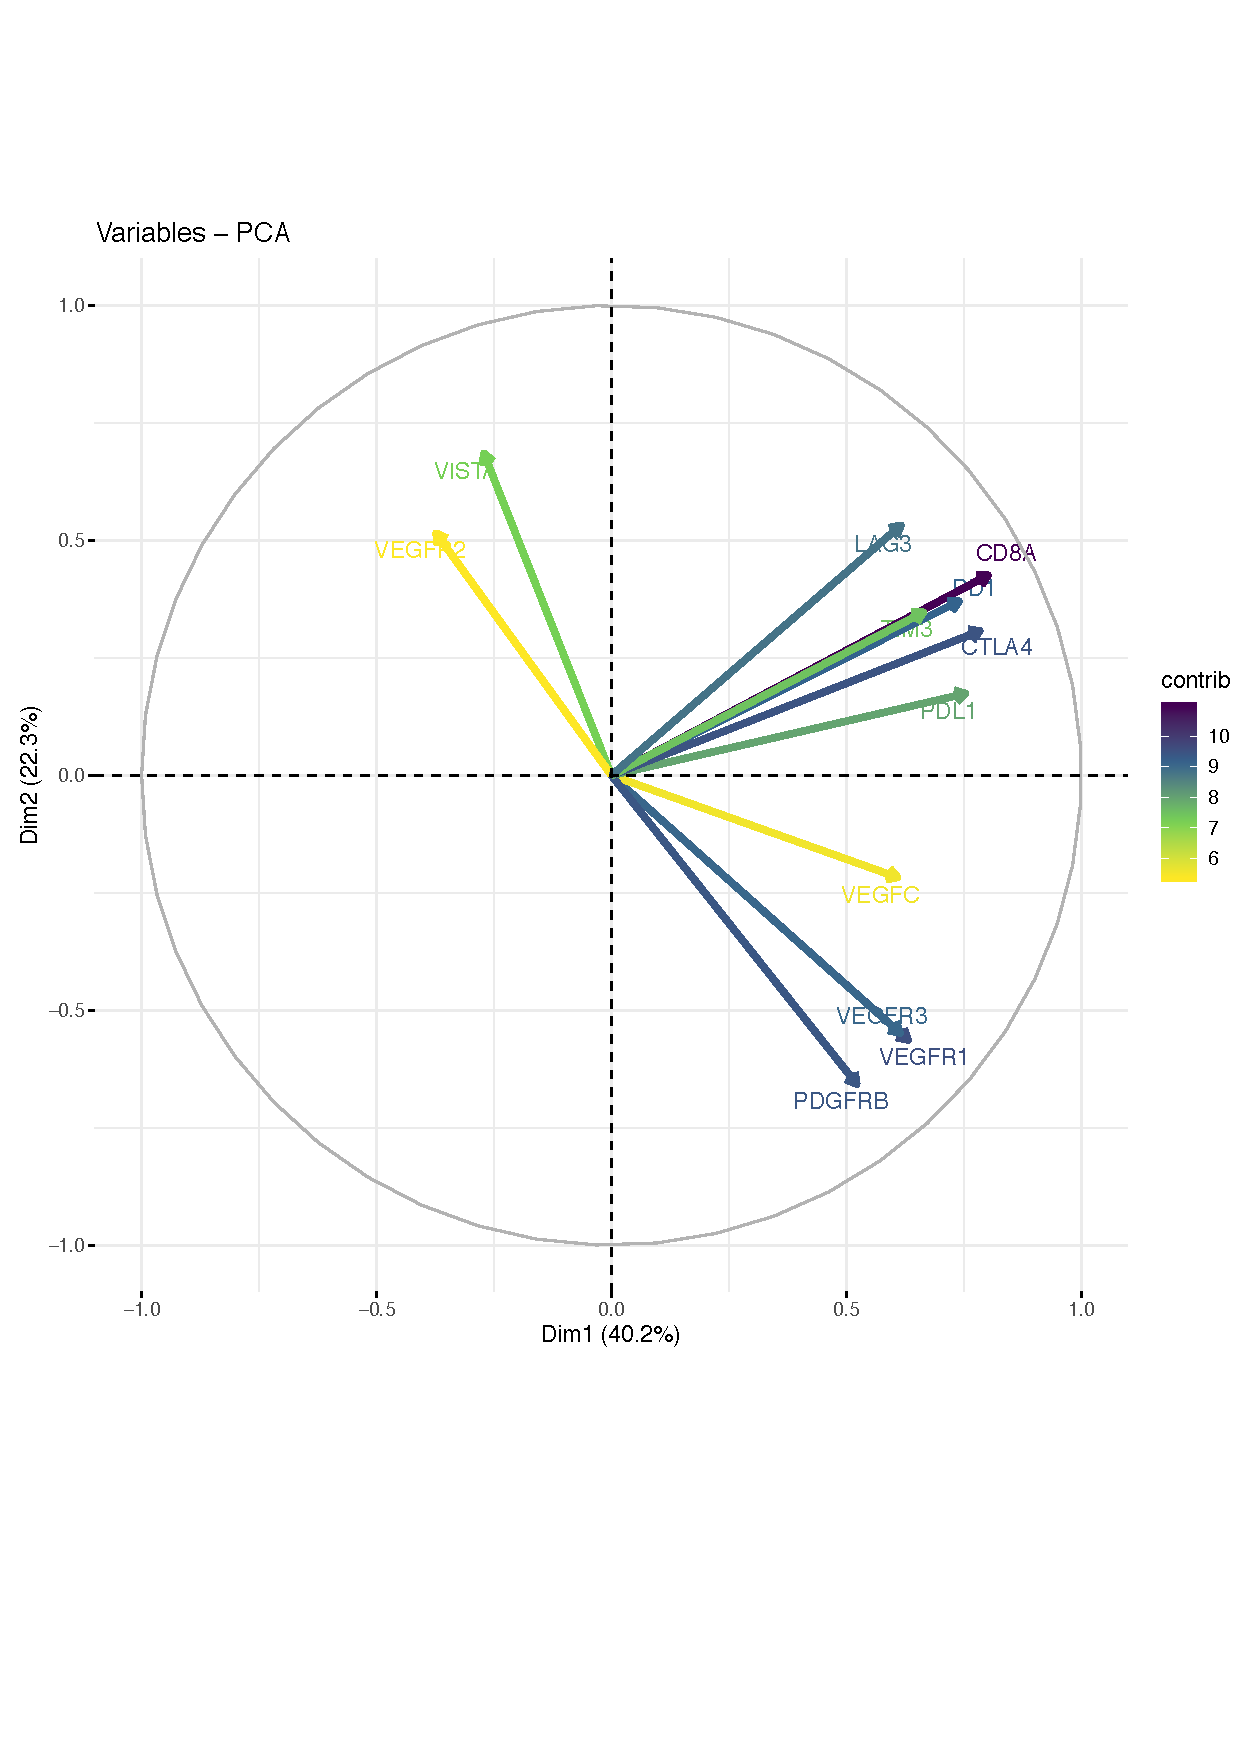
\includegraphics[height=7cm]{figures/methods/COR_CIRCLE.pdf}
  \end{figure}
  \end{column}
 \end{columns} 
  
 
  
     \onslide<3>
\begin{columns}[c]
  \begin{column}{0.55\linewidth}
 \begin{itemize}
     \item \textbf{Structure preservation : }\\
     \begin{itemize}
         \item Centrality 
         \item Neighborhood
     \end{itemize}
 \end{itemize}
  \begin{itemize}
    \item   \textbf{Correlations' consistency : }\\
     \begin{itemize}
         \item Control of dataset's noise
         \item Highlighting key features 
     \end{itemize}
\end{itemize}
 \begin{itemize}
    \item   \textbf{Clusters' relevance : }\\
     \begin{itemize}
         \item Explained variance
         \item Highlighting key features 
     \end{itemize}
\end{itemize}

  \end{column}
  \begin{column}{0.45\linewidth}
\begin{figure}
\centering
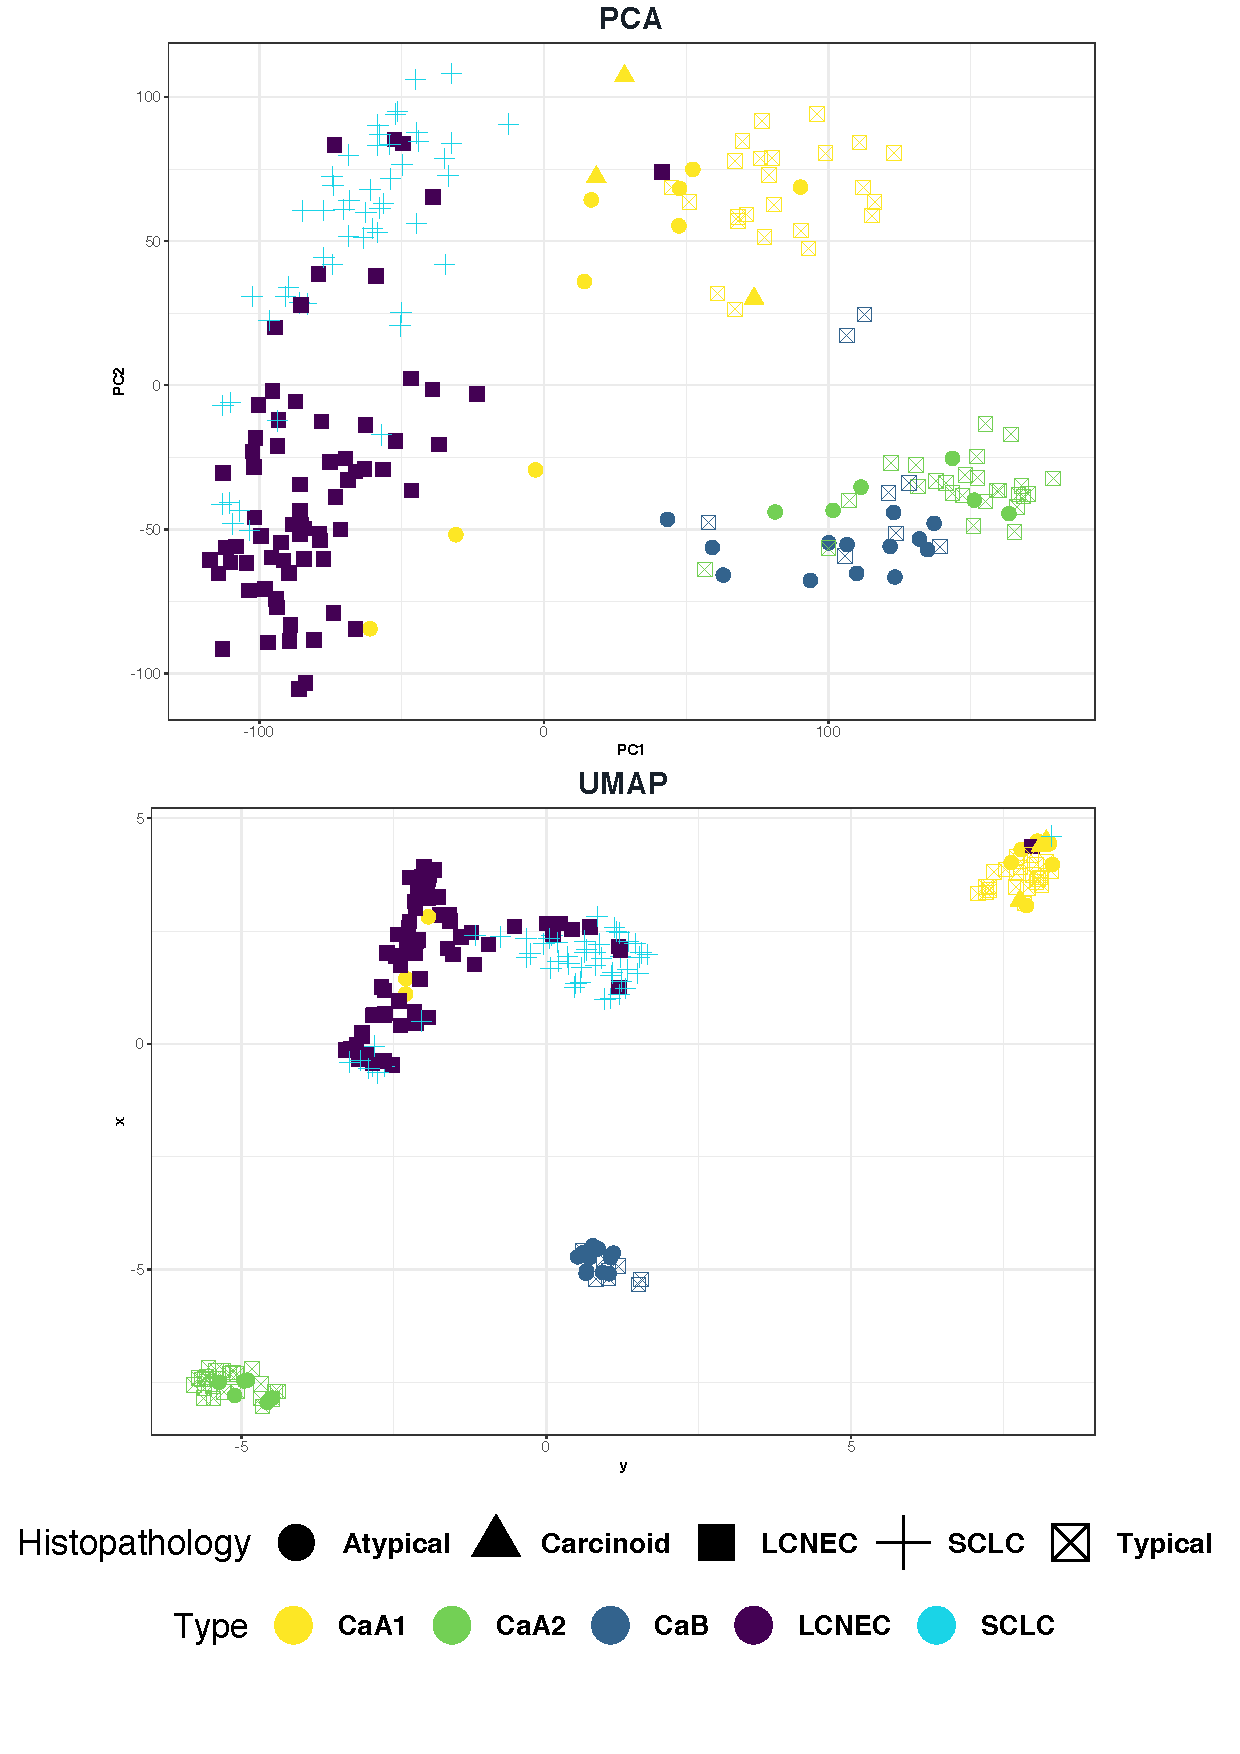
\includegraphics[height=7cm]{figures/methods/PCA_UMAP2.pdf}
  \end{figure}
  \end{column}
 \end{columns} 
  
\end{overprint}

  \begin{flushright}
\color{IARCdblue}{ \scriptsize{\insertframenumber / \inserttotalframenumber}} \hspace*{2mm}
  \end{flushright}

\end{frame}



%%%%%%%%%%%%%%%%%%%%%%%%%%%%%%%%%%%%%%%%%%%%%%%%%%

%%%%%%%%%%%%%%%%%%%%%%%%%%%%%%%%%%%%%%%%%%%%%%%%%
\section{Results : Centrality preservation}
\begin{frame}
\vspace*{-1cm}
\begin{figure}
    \centering
    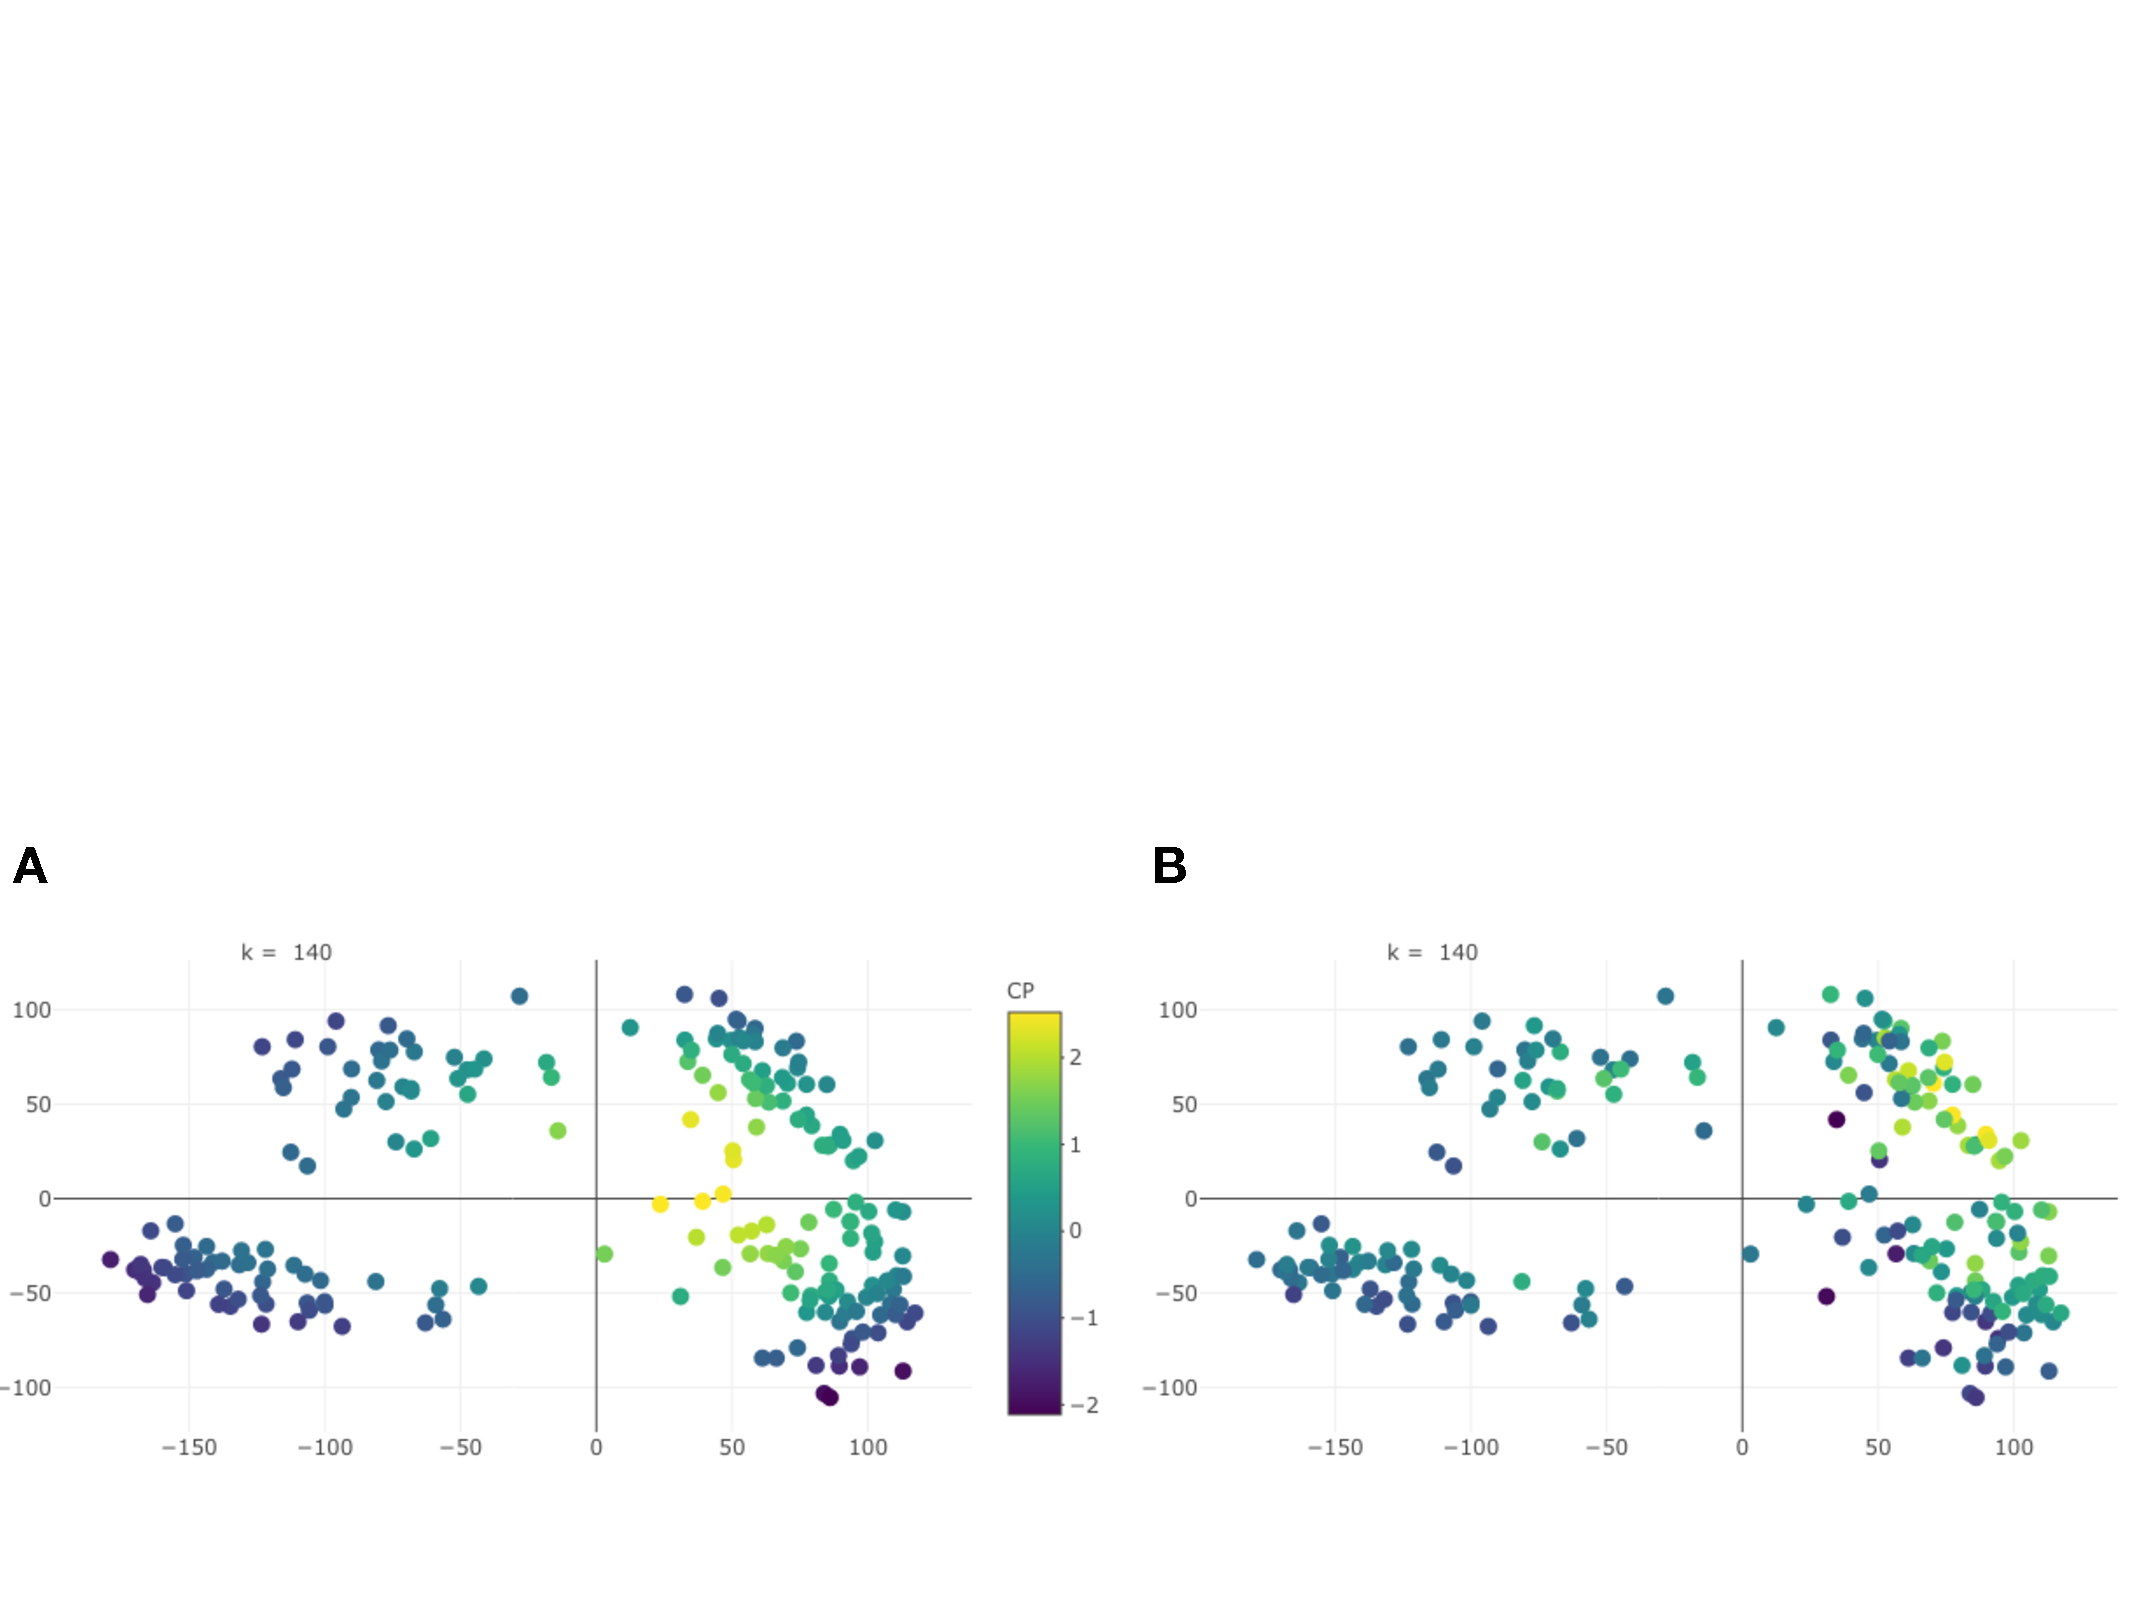
\includegraphics[width = \linewidth]{figures/results/results_map.pdf}
\end{figure}

\textbf{A)} CP values \textbf{calculated on PCA}  and  \textbf{projected on PCA} layout. \\
\textbf{B)} CP values calculated  on genes expression data frame projected on PCA layout. 
\textbf{A)} CP values \textbf{calculated on PCA}  and  \textbf{projected on PCA} layout. \\

  \begin{flushright}
\color{IARCdblue}{ \scriptsize{\insertframenumber / \inserttotalframenumber}} \hspace*{2mm}
  \end{flushright}

\end{frame}





%%%%%%%%%%%%%% BIBLIO %%%%%%%%%%%%%%%%%%%%%%%%%%%%%%%%%%%%%%%%%%%%%
\section{References}
\subsection{}
\begin{frame}[shrink=40, noframenumbering]
\bibliography{sample.bib} % Add the filename of your bibliography
\tiny\bibliographystyle{ieeetr} % Defines
\end{frame}





\end{document}
